%----------------------------------------------------------------------------------------
%	PACKAGES AND OTHER DOCUMENT CONFIGURATIONS
%----------------------------------------------------------------------------------------
 
\documentclass[12pt]{article}
    \usepackage{graphicx} %Needed for logos
    \usepackage{tikz}
    \usetikzlibrary{matrix,calc} 
    \usepackage{fancyhdr}
    \pagestyle{fancy}
    \fancyhead[L]{Left}
    \fancyhead[R]{Right} 
    \fancyhead[C]{Center}
    \usepackage{lastpage}
    \usepackage{float}
    \usepackage{amsmath}
    \usepackage{enumerate,letltxmacro}
    \LetLtxMacro\itemold\item
    \renewcommand{\item}{\itemindent1cm\itemold}
    \usepackage{enumitem} 
    \usepackage{verbatim} 
    \usepackage[english]{babel}
    \usepackage{blindtext}
    \usepackage{varwidth}
    \setlength\parindent{24pt}
    \usepackage{booktabs} 
    \usepackage{tabularx}
    \newcolumntype{C}{>{\centering\arraybackslash}X}
    \usepackage{bm}  
    \usepackage[object=vectorian]{pgfornament} 
    \usepackage{tikzpagenodes}
    \usepackage{lipsum}
    \usepackage{booktabs,pdflscape,adjustbox} 
    \usepackage{abstract}
    \usepackage{setspace}
    \usepackage{ragged2e}
    \usepackage{listings}
    \usepackage{color, xcolor}
    \usepackage{fancybox}
    \usepackage{hyperref}
    \usepackage{fontawesome}
    \usepackage{subcaption}
    \usetikzlibrary{arrows,positioning,automata}
    \usepackage{tkz-graph}
    \usepackage{amsfonts}
    \usepackage[toc,page]{appendix}
    \usepackage{gensymb}

    \usepackage[margin=0.95in]{geometry}
    
    %----------------------------------------------------------------------------------------
    %	TITLE PAGE
    %----------------------------------------------------------------------------------------
    
    \newcommand*{\titleGP}{\begingroup % Create the command for including the title page in the document
    \centering % Center all text
    \vspace*{\baselineskip} % White space at the top of the page
    \vspace*{-1.0cm}
    \centerline{\rule{17cm}{1.6pt}}\vspace*{-\baselineskip}\vspace*{2pt} % Thick horizontal line
    \centerline{\rule{17cm}{0.4pt}}\ \\[\baselineskip] % Thin horizontal line
    
    {\LARGE 16:332:599:02 -- Smart Grid \\ \vspace*{0.2cm}\Large Project Report \vspace*{0.2cm}\small \\By David Lambropoulos, Demetrios Lambropoulos}
    % Title 
    
    \centerline{\rule{17cm}{0.4pt}}\vspace*{-\baselineskip}\vspace{3.2pt} % Thin horizontal line
    \centerline{\rule{17cm}{1.6pt}}\ \\[\baselineskip] % Thick horizontal line
    \vspace*{-0.35cm}Professor Hana Godrich\par
    May $\text{9}^\text{th}$, 2018\par
    \vfill 
    \vspace*{10.3cm}
    \centerline{
\includegraphics[scale=0.5]{images/rulogo}} 
    \textit{Rutgers University}\par
    \textit{School of Engineering}\par
    
    \vspace*{2\baselineskip} % Whitespace between location/year and editors
    
    \vfill % Whitespace between editor names and publisher logo
    
        
    \endgroup}
    
    %----------------------------------------------------------------------------------------
    %   CENTERED BOX
    %----------------------------------------------------------------------------------------
    \makeatletter
    \newenvironment{CenteredBox}{% 
    \begin{Sbox}}{% Save the content in a box
    \end{Sbox}\centerline{\parbox{\wd\@Sbox}{\TheSbox}}}% And output it centered
    \makeatother
        
        
    %----------------------------------------------------------------------------------------
    %   LSTLISTING CODE DEFINITION
    %----------------------------------------------------------------------------------------
    \definecolor{codegreen}{rgb}{0,0.6,0}
    \definecolor{codegray}{rgb}{0.5,0.5,0.5}
    \definecolor{codepurple}{rgb}{0.58,0,0.82}
    \definecolor{backcolour}{rgb}{0.95,0.95,0.92}
        
    \lstdefinestyle{mystyle}{
        backgroundcolor=\color{backcolour},   
        commentstyle=\color{codegreen},
        keywordstyle=\color{magenta},
        numberstyle=\tiny\color{codegray},
        stringstyle=\color{codepurple},
        basicstyle=\footnotesize,
        breakatwhitespace=false,         
        breaklines=true,                 
        captionpos=b,                    
        keepspaces=true,                 
        numbers=left,                    
        numbersep=5pt,                  
        showspaces=false,                
        showstringspaces=false,
        showtabs=false,                  
        tabsize=4
    }
    
    %----------------------------------------------------------------------------------------
    %	BUILD HEADER
    %----------------------------------------------------------------------------------------
    
    % Length to control the \fancyheadoffset and the calculation of \headline
    % simultaneously
    \newlength\FHoffset
    \setlength\FHoffset{1cm}
    
    \addtolength\headwidth{2\FHoffset}
    
    \fancyheadoffset{\FHoffset}
    
    % these lengths will control the headrule trimming to the left and right  
    \newlength\FHleft
    \newlength\FHright
    
    % here the trimmings are controlled by the user
    \setlength\FHleft{1cm} 
    \setlength\FHright{0cm}
    
    % The new definition of headrule that will take into acount the trimming(s)
    \newbox\FHline
    \setbox\FHline=\hbox{\hsize=\paperwidth%
        \hspace*{\FHleft}%
        \rule{\dimexpr\headwidth-\FHleft-\FHright\relax}{\headrulewidth}\hspace*{\FHright}%
    }
    \renewcommand\headrule{} 
    
    
    %----------------------------------------------------------------------------------------
    %	BODY OF DOCUMENT
    %----------------------------------------------------------------------------------------
    
    \begin{document}    
        \pagestyle{empty} % Removes page numbers 
        \onecolumn
        \titleGP % This command includes the title page
        \newpage
        \renewcommand*\contentsname{Contents}
        \tableofcontents
        \newpage

        \listoffigures
        \newpage

        \listoftables
        \newpage 
        
        \setcounter{page}{1}
        \pagestyle{fancy}
        \lhead{David, Demetrios\\} 
        \chead{NetID: dal220, dpl60\\ \myrule} 
        \rhead{16:332:599:02 -- Smart Grid\\ \myrule}
        \lfoot{\vspace*{-0.1cm}\myrule \\ \vspace*{0.1cm}Project Report}
        \cfoot{}
        \rfoot{\vspace*{-0.1cm}\myrule \\\vspace*{0.1cm}Page - \thepage{} }
        
        \newcommand\myrule{%
            \leavevmode\cleaders\hbox{\raisebox{-2.5pt}{\pgfornament[width=0.2\textwidth]{88}}}\hfill\kern0pt}

        \section{Case Study/Problem Formulation}
        For the single-line diagram in Figure 4 convert all positive-sequence impedance, load,
        and voltage data to per unit using the given system base quantities.
        Run the power flow program and obtain the bus, line, and transformer input/output
        voltages 

        \begin{figure}[H]
            \centerline{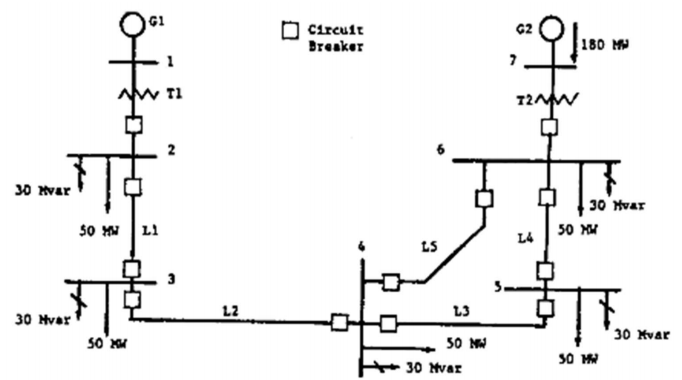
\includegraphics[scale=0.565]{images/problemCircuit}}
            \caption{Original Circuit}
        \end{figure}

        \begin{table}[H]
            \centering
            \begin{tabular}{|c|p{13cm}|}
                \hline
                \multicolumn{2}{|c|}{\textbf{Generator Ratings}}\\\hline
                \textbf{G1}&$100MVA$, $13.8kV$, $x^{''}=0.12$\\\hline
                \textbf{G2}&$200MVA$, $15.0kV$, $x^{''}=0.12$\\\hline
                \multicolumn{2}{|c|}{\textit{The generator neutrals are solidly grounded}}\\\hline
                \multicolumn{2}{c}{}\\\hline
                \multicolumn{2}{|c|}{\textbf{Transformer Ratings}}\\\hline
                \textbf{T1}&$100MVA$, $13.8kV\Delta/230 kVY$, $x=0.1$ per unit\\\hline
                \textbf{T2}&$200MVA$, $15kV\Delta/230 kVY$, $x=0.1$ per unit\\\hline
                \multicolumn{2}{|c|}{\textit{The transformer neutrals are solidly grounded}}\\\hline
                \multicolumn{2}{c}{}\\\hline
                \multicolumn{2}{|c|}{\textbf{Transmission Line Ratings}}\\\hline
                \textbf{All Lines}&$230kV$, $z_1=0.08+j0.5\Omega/km$, $y_1=j3.3E-6 S/km$, $Max\ MVA=400$\\\hline
                \textbf{Line Lengths}&$L_1=15km$, $L_2=20km$, $L_3=40km$, $L_4=15km$, $L_5=50km$\\\hline
                \multicolumn{2}{c}{}\\\hline
                \multicolumn{2}{|c|}{\textbf{Power Flow Data}}\\\hline
                \textbf{Bus 1}&Swing bus $V_1=13.8kV$, $\partial_1=0\degree$\\\hline
                \textbf{Bus 2, 3, 4, 5, 6}&Load buses\\\hline
                \textbf{Bus 7}&Constant voltage magnitude bus, $V_7=15kV$, $P_{G7}=180MW$, $-87MVAr<Q_{G7}<+87MVAr$\\\hline
                \multicolumn{2}{c}{}\\\hline
                \multicolumn{2}{|c|}{\textbf{System Base Quantities}}\\\hline
                \multicolumn{2}{|c|}{$S_{base}=100MVA$ (three-phase)}\\\hline
                \multicolumn{2}{|c|}{$V_{base}=13.8kV$ (line-to-line) in the zone of $G_1$}\\\hline
            \end{tabular}
            \caption{Circuit Values}
        \end{table}
        \newpage
        \section{Detailed Solution}
        \subsection{Calculating Per Unit Values}
        $$per\ unit\ (pu)\ value=\frac{Actual\ value}{Base\ value}$$
        
        
        In zone $G1$, base values are,
        $$S_{base}=100MVA$$
        $$V_{base_{L-L}}=13.8kV$$
        
        \ \\
        @ $G1$
        $$S_{G1_{(pu)}}=\frac{100MVA}{100MVA}=\boxed{1pu}$$
        $$V_{G1_{(pu)}}=\frac{13.8kV}{13.8kV}=\boxed{1pu}$$
        $$x^{''}_{(new)}=\boxed{0.12pu}$$

        \ \\
        @ $T1$
        $$S_{T1_{(pu)}}=\frac{100MVA}{100MVA}=\boxed{1pu}$$
        $$V_{T1_{(pu)}}=\frac{13.8kV}{13.8kV}=\boxed{1pu}$$
        $$x_{(pu)}=\boxed{0.1pu}$$

        \ \\
        @ Bus 2
        $$Q_{Load}=30MVAr$$
        $$Q_{Load_{(pu)}}=\frac{30MVAr}{100MVA}=\boxed{0.3pu}$$
        
        $$P_{Load}=50MW$$
        $$P_{Load_{(pu)}}=\frac{50MW}{100MVA}=\boxed{0.5pu}$$

        \ \\
        @ $L_1$
        $$L_1=15km$$
        $$z=0.08+j0.5\Omega/km$$
        $$Z_{total}=(15km)(0.08+j0.5\Omega/km)=\boxed{1.2+j7.5\Omega}$$
        $$\theta=tan^{-1}\left(\frac{7.5}{1.2}\right)=\boxed{80.91\degree}$$
        $$|Z_{total}|=\sqrt{(1.2)^2+(7.5)^2}=\boxed{7.59539\Omega}$$
        $$Z_{total}=\boxed{7.59539\angle80.91\degree\Omega}$$
        $$Z_{total_{(pu)}}=7.595\cdot\left(\frac{100MVA}{(230kV)^2}\right)=\boxed{0.014358pu}$$

        \ \\
        @ Bus 3
        $$Q_{Load}=30MVAr$$
        $$Q_{Load_{(pu)}}=\frac{30MVAr}{100MVA}=\boxed{0.3pu}$$
        
        $$P_{Load}=50MW$$
        $$P_{Load_{(pu)}}=\frac{50MW}{100MVA}=\boxed{0.5pu}$$
        
        \ \\
        @ Bus 4
        $$Q_{Load}=30MVAr$$
        $$Q_{Load_{(pu)}}=\frac{30MVAr}{100MVA}=\boxed{0.3pu}$$
        
        $$P_{Load}=50MW$$
        $$P_{Load_{(pu)}}=\frac{50MW}{100MVA}=\boxed{0.5pu}$$
        
        \ \\
        @ Bus 5
        $$Q_{Load}=30MVAr$$
        $$Q_{Load_{(pu)}}=\frac{30MVAr}{100MVA}=\boxed{0.3pu}$$
        
        $$P_{Load}=50MW$$
        $$P_{Load_{(pu)}}=\frac{50MW}{100MVA}=\boxed{0.5pu}$$
        
        \ \\
        @ Bus 6
        $$Q_{Load}=30MVAr$$
        $$Q_{Load_{(pu)}}=\frac{30MVAr}{100MVA}=\boxed{0.3pu}$$
        
        $$P_{Load}=50MW$$
        $$P_{Load_{(pu)}}=\frac{50MW}{100MVA}=\boxed{0.5pu}$$

        \ \\
        @ $L_2$
        $$L_2=20km$$
        $$z=0.08+j0.5\Omega/km$$
        $$Z_{total}=(20km)(0.08+j0.5\Omega/km)=\boxed{1.6+j10\Omega}$$
        $$\theta=tan^{-1}\left(\frac{10}{1.6}\right)=\boxed{80.91\degree}$$
        $$|Z_{total}|=\sqrt{(1.6)^2+(10)^2}=\boxed{10.127191\Omega}$$
        $$Z_{total}=\boxed{10.127191\angle80.91\degree\Omega}$$
        $$Z_{total_{(pu)}}=10.127191\cdot\left(\frac{100MVA}{(230kV)^2}\right)=\boxed{0.019144pu}$$

        \ \\
        @ $L_3$
        $$L_3=40km$$
        $$z=0.08+j0.5\Omega/km$$
        $$Z_{total}=(40km)(0.08+j0.5\Omega/km)=\boxed{3.2+j20\Omega}$$
        $$\theta=tan^{-1}\left(\frac{20}{3.2}\right)=\boxed{80.91\degree}$$
        $$|Z_{total}|=\sqrt{(3.2)^2+(20)^2}=\boxed{20.254382\Omega}$$
        $$Z_{total}=\boxed{20.254382\angle80.91\degree\Omega}$$
        $$Z_{total_{(pu)}}=20.254382\cdot\left(\frac{100MVA}{(230kV)^2}\right)=\boxed{0.038288pu}$$

        \ \\
        @ $L_4$
        $$L_4=15km$$
        $$z=0.08+j0.5\Omega/km$$
        $$Z_{total}=(15km)(0.08+j0.5\Omega/km)=\boxed{1.2+j7.5\Omega}$$
        $$\theta=tan^{-1}\left(\frac{7.5}{1.2}\right)=\boxed{80.91\degree}$$
        $$|Z_{total}|=\sqrt{(1.2)^2+(7.5)^2}=\boxed{7.59539\Omega}$$
        $$Z_{total}=\boxed{7.59539\angle80.91\degree\Omega}$$
        $$Z_{total_{(pu)}}=7.595\cdot\left(\frac{100MVA}{(230kV)^2}\right)=\boxed{0.014358pu}$$

        \ \\
        @ $L_5$
        $$L_5=50km$$
        $$z=0.08+j0.5\Omega/km$$
        $$Z_{total}=(50km)(0.08+j0.5\Omega/km)=\boxed{4+j25\Omega}$$
        $$\theta=tan^{-1}\left(\frac{25}{4}\right)=\boxed{80.91\degree}$$
        $$|Z_{total}|=\sqrt{(4)^2+(25)^2}=\boxed{25.317978\Omega}$$
        $$Z_{total}=\boxed{25.317978\angle80.91\degree\Omega}$$
        $$Z_{total_{(pu)}}=25.317978\cdot\left(\frac{100MVA}{(230kV)^2}\right)=\boxed{0.04786pu}$$

        \ \\
        @ Bus 7
        $$P_{G7_{(pu)}}=\frac{180MW}{100MVA}=\boxed{1.8pu}$$
        $$\frac{-87MVAr}{100}<Q_{G7_{(pu)}}<\frac{87MVAr}{100}$$
        $$-0.87pu<Q_{G7_{(pu)}}<0.87pu$$
        $$V_{T2_{(pu)}}=\frac{15kV}{13.8kV}=\boxed{1.086956pu}$$
        
        \subsubsection{Per-Unit One-Line Model}
        \begin{figure}[H]
            \centerline{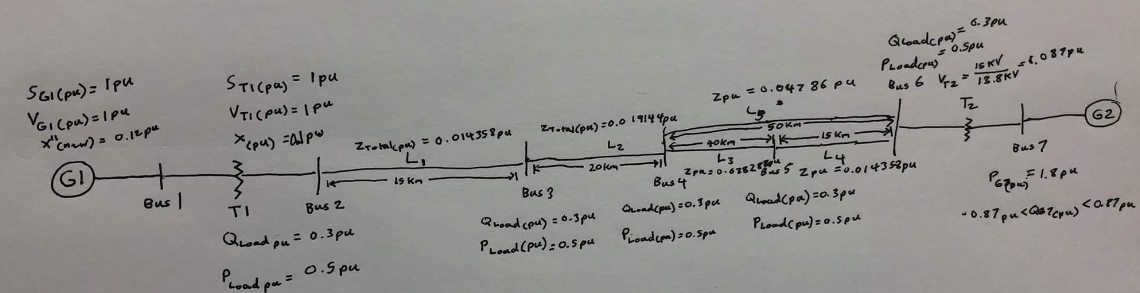
\includegraphics[scale=0.5]{images/oneLine}}
            \caption{Per-Unit One-line Diagram}
        \end{figure}

        \subsection{Compute All Bus Voltages}
        \begin{figure}[H]
            \centerline{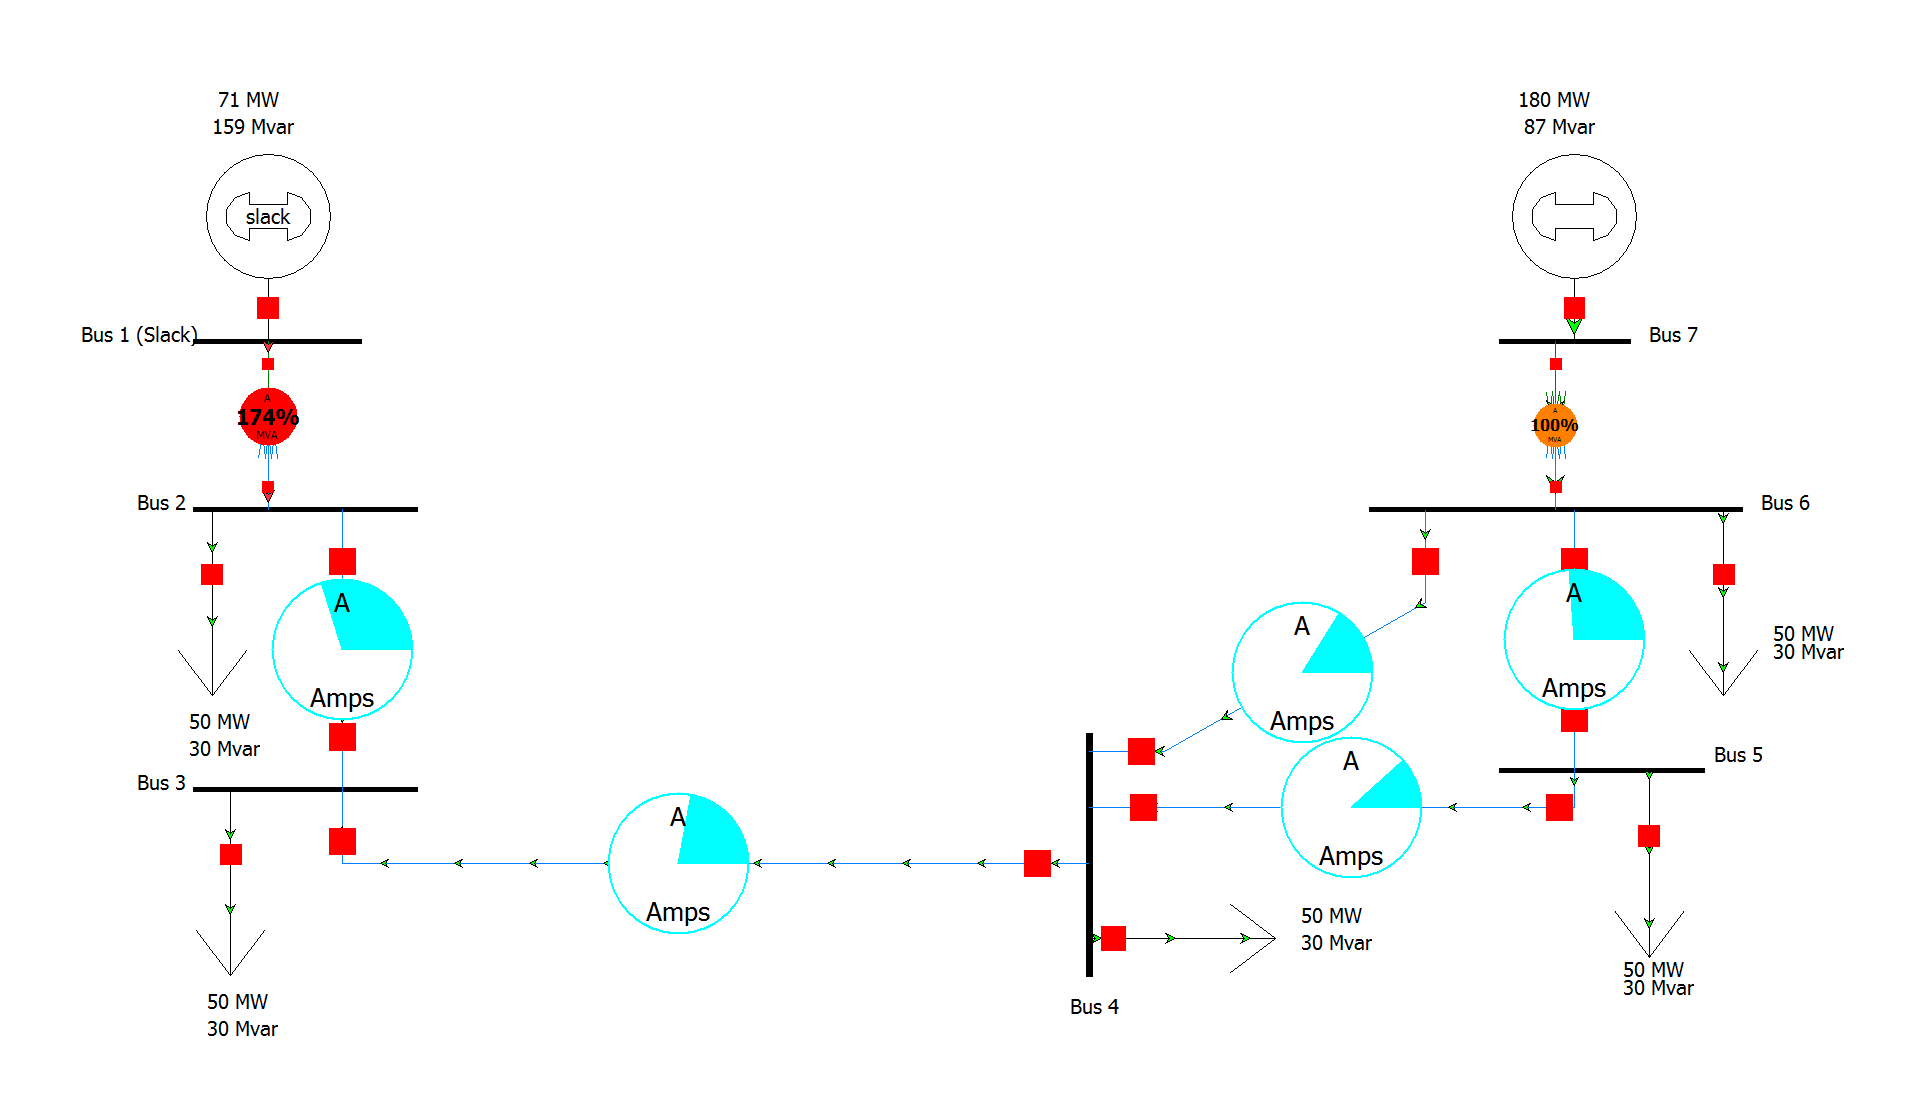
\includegraphics[scale=0.3]{images/PowerWorld}}
            \caption{PowerWorld Diagram - Full Powerflow Analysis}
        \end{figure}
        
        \subsubsection{Newton-Raphson Method}
        \begin{figure}[H]
            \centerline{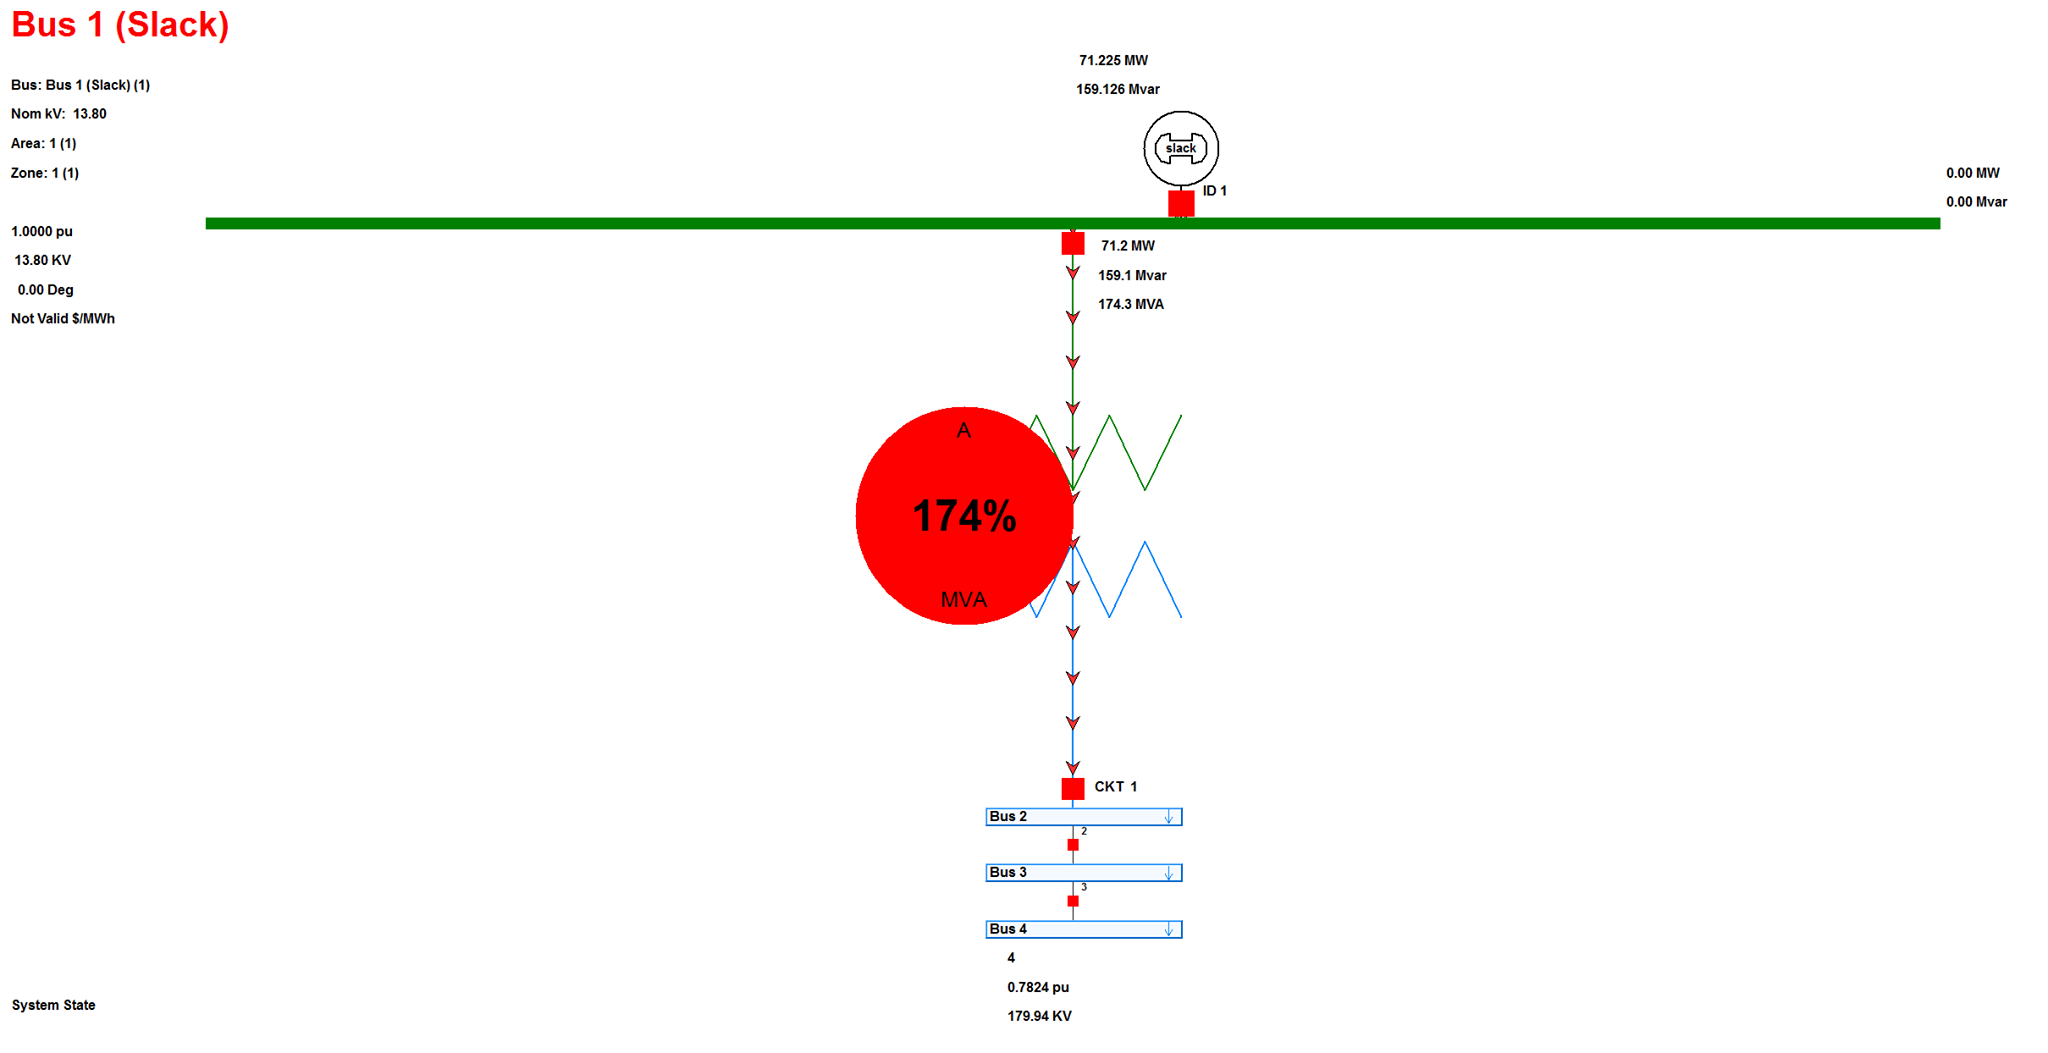
\includegraphics[scale=0.25]{images/PowerWorldBus1}}
            \caption{PowerWorld Diagram - Bus 1 after Newton-Raphson}
        \end{figure}

        \begin{figure}[H]
            \centerline{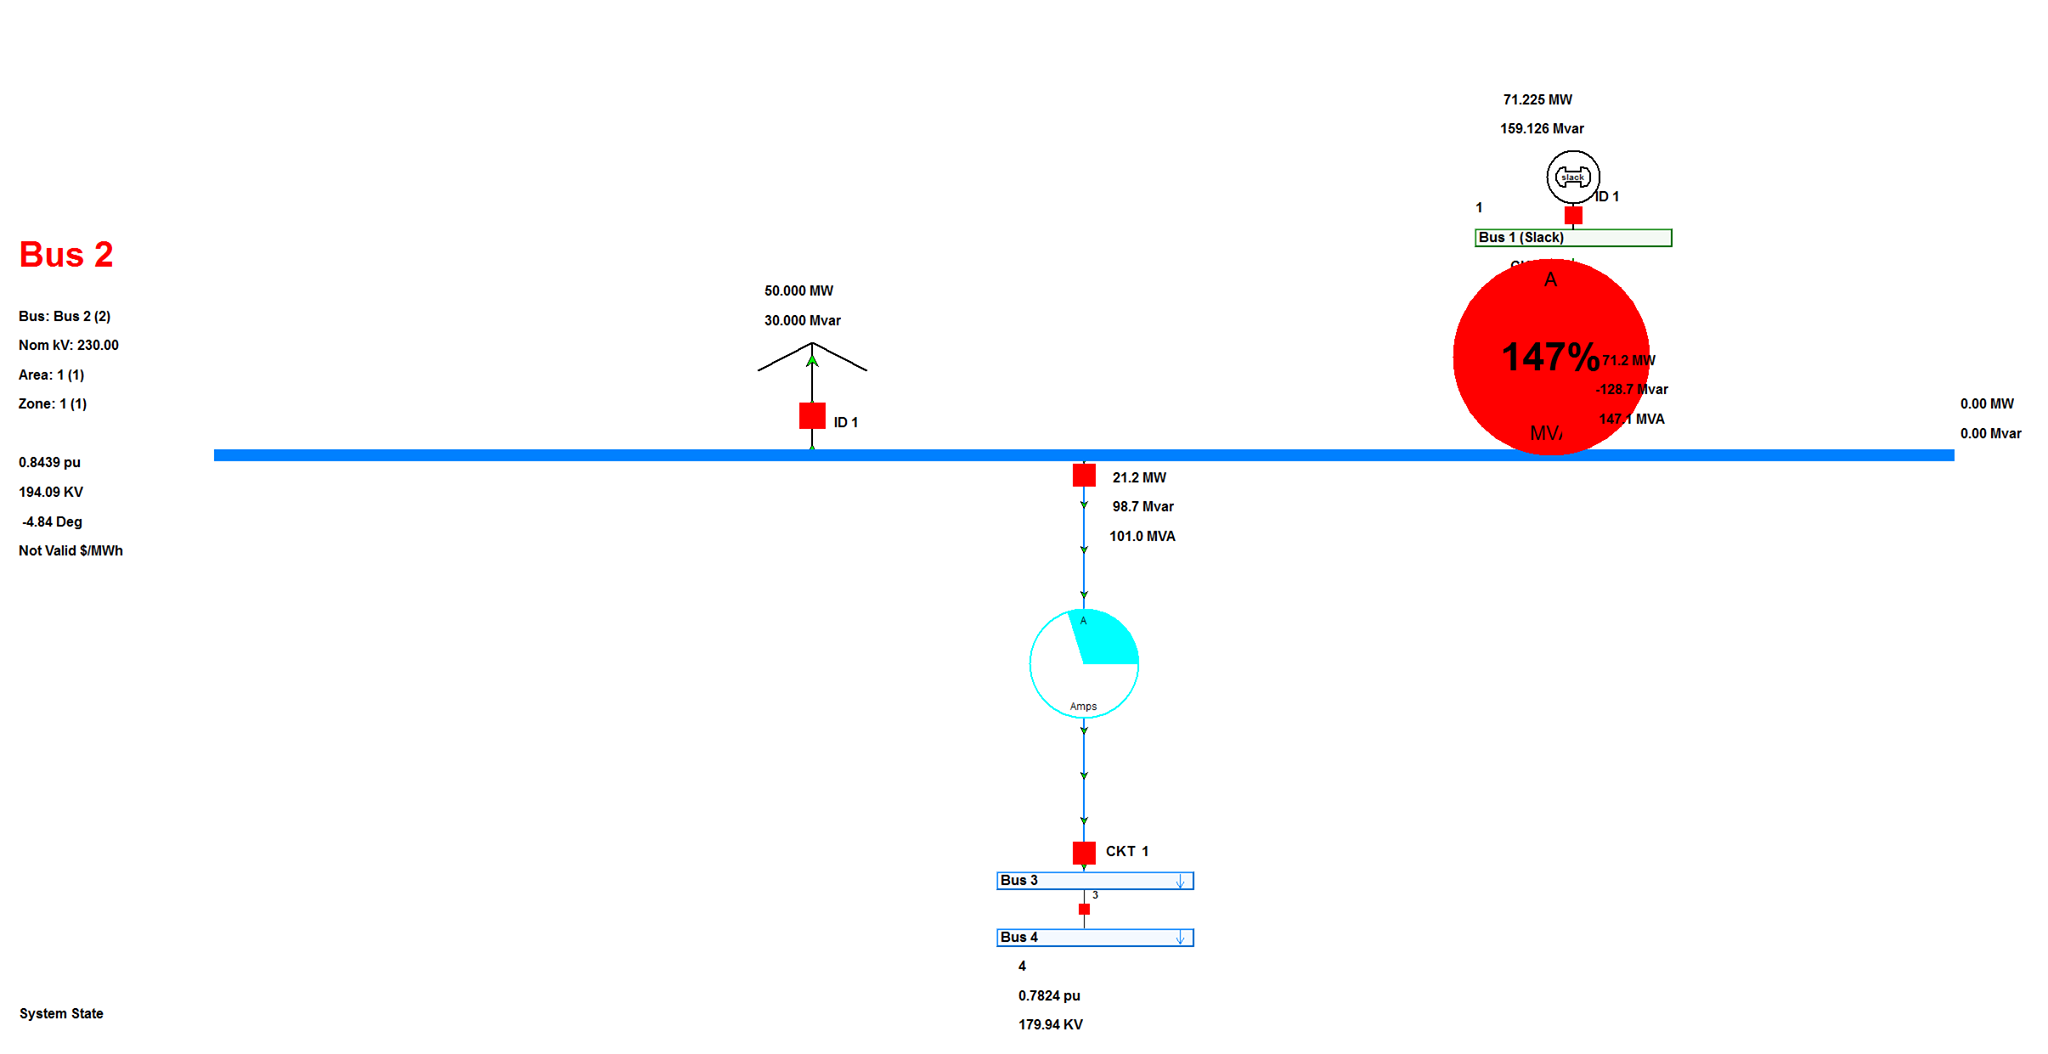
\includegraphics[scale=0.25]{images/PowerWorldBus2}}
            \caption{PowerWorld Diagram - Bus 2 after Newton-Raphson}
        \end{figure}

        \begin{figure}[H]
            \centerline{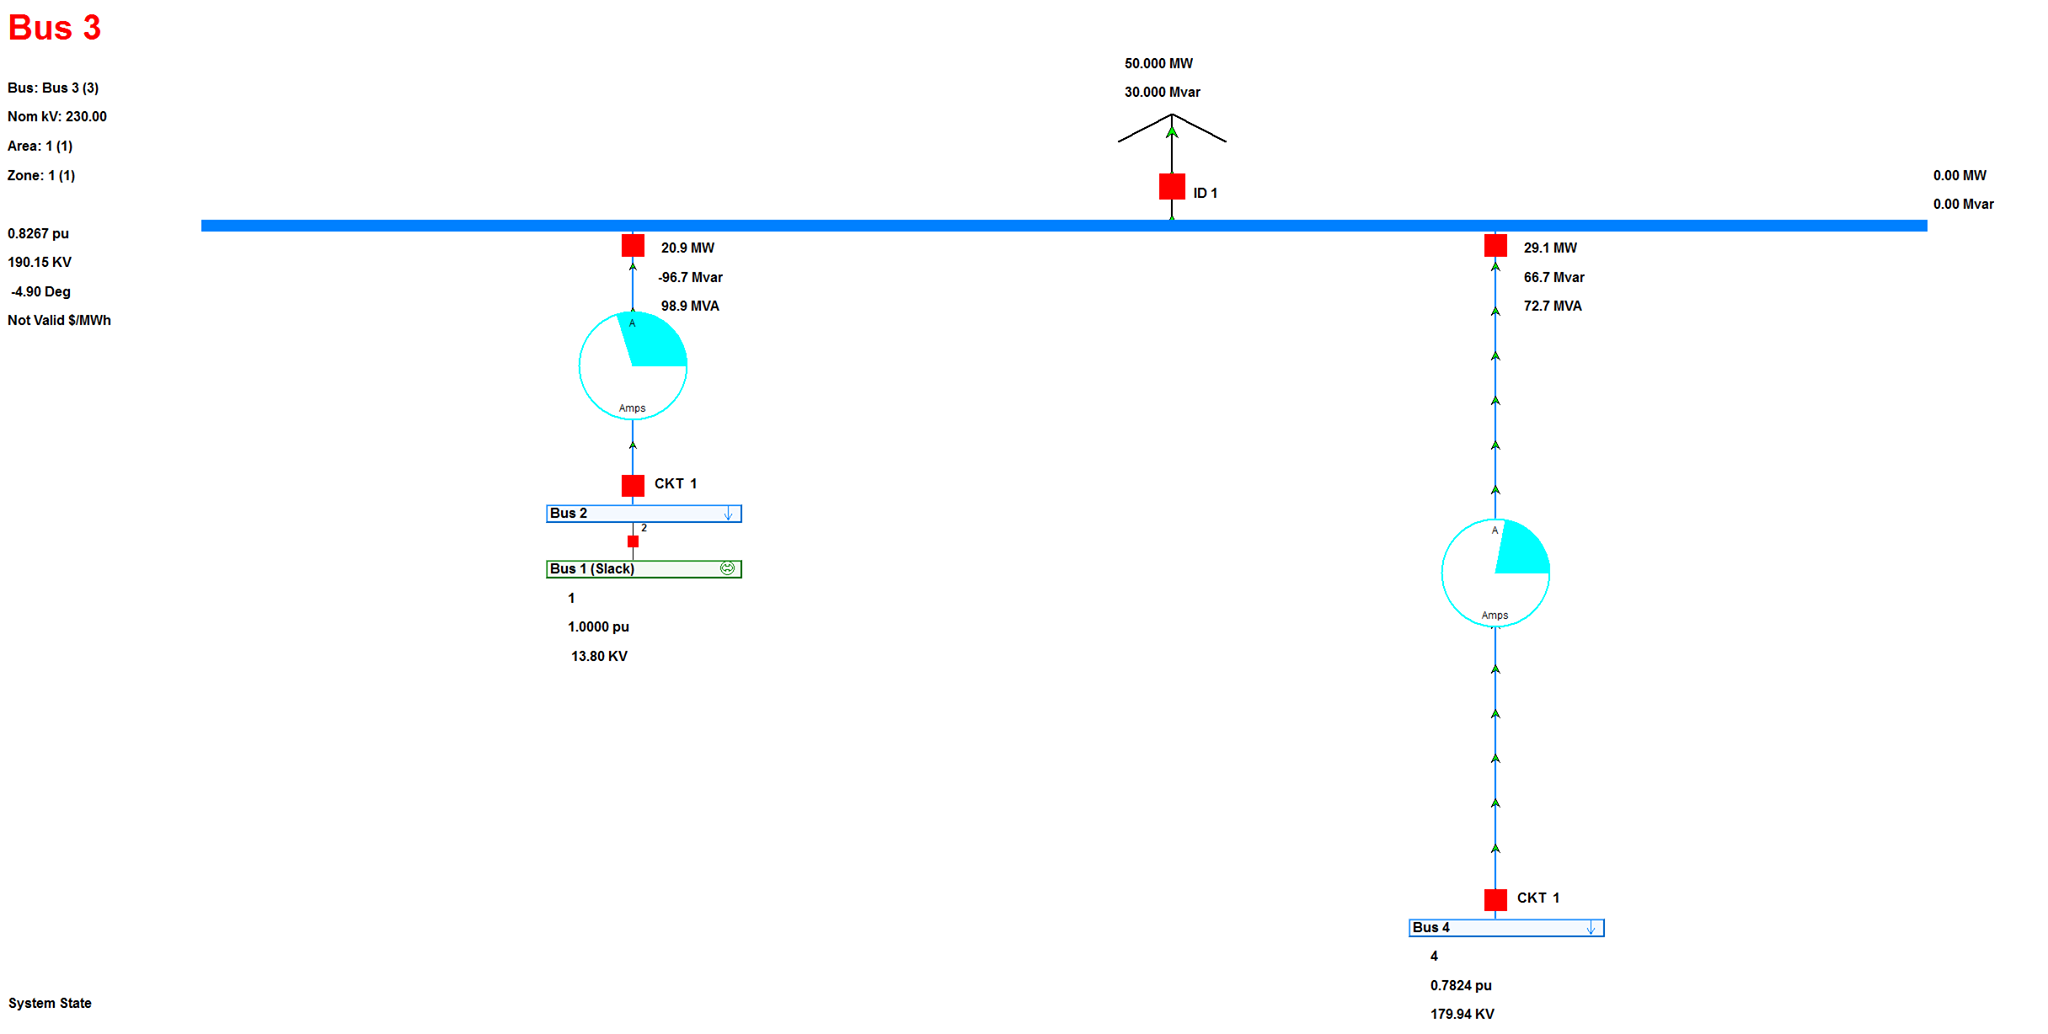
\includegraphics[scale=0.25]{images/PowerWorldBus3}}
            \caption{PowerWorld Diagram - Bus 3 after Newton-Raphson}
        \end{figure}

        \begin{figure}[H]
            \centerline{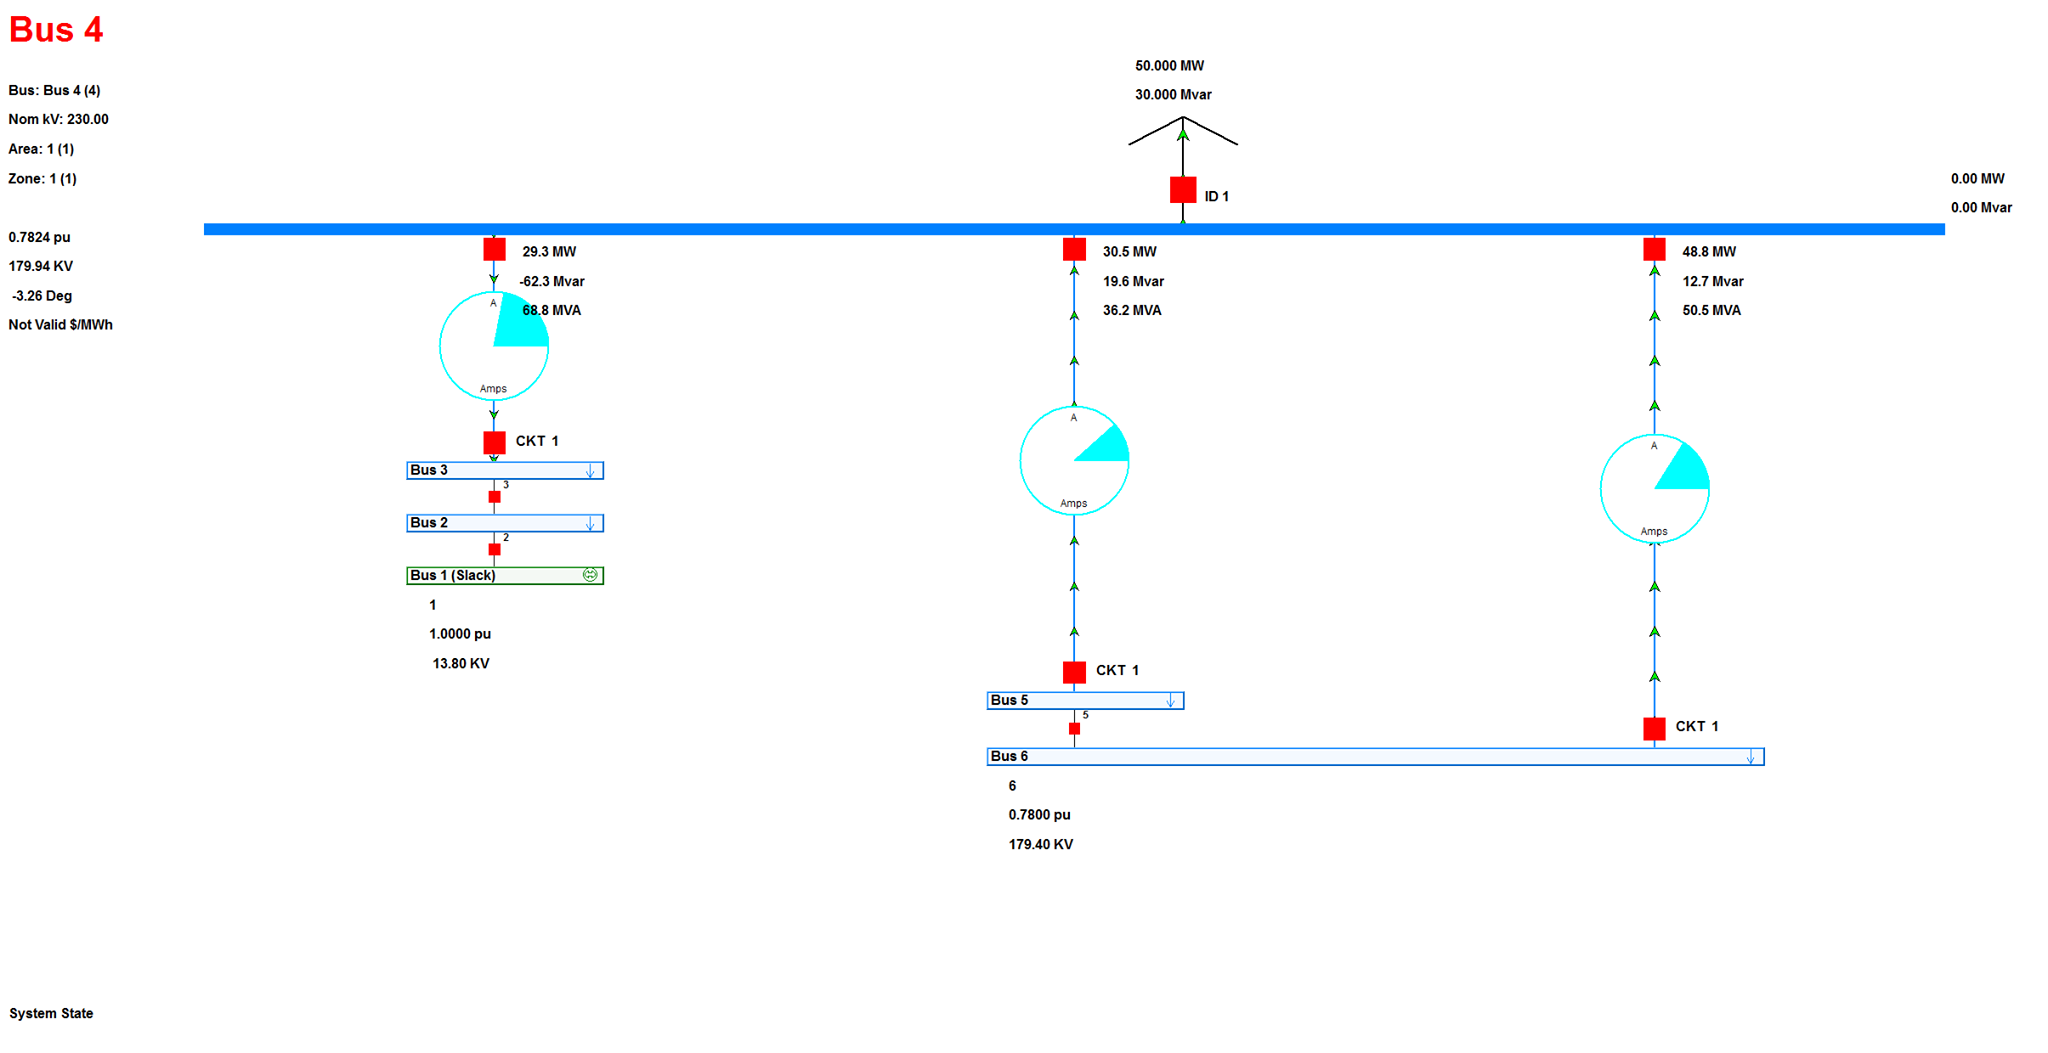
\includegraphics[scale=0.25]{images/PowerWorldBus4}}
            \caption{PowerWorld Diagram - Bus 4 after Newton-Raphson}
        \end{figure}

        \begin{figure}[H]
            \centerline{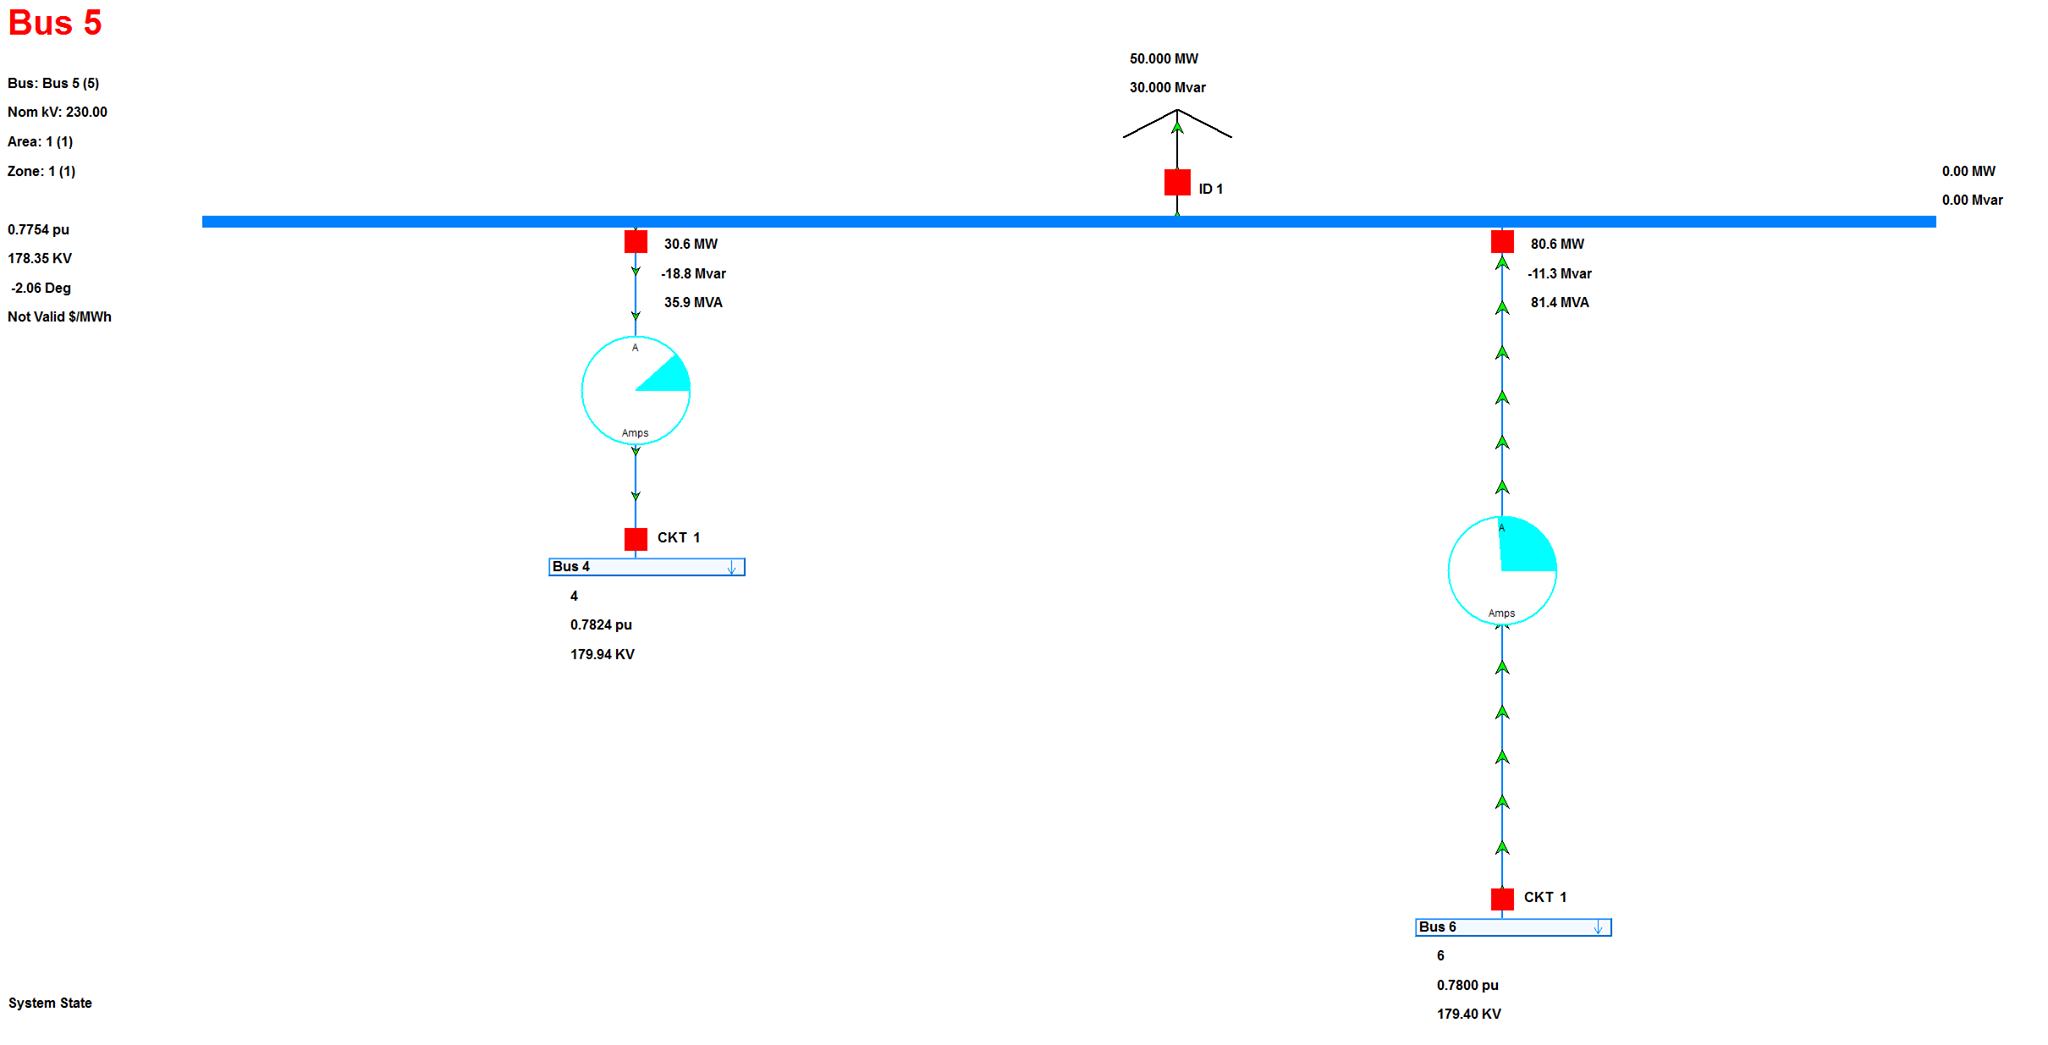
\includegraphics[scale=0.25]{images/PowerWorldBus5}}
            \caption{PowerWorld Diagram - Bus 5 after Newton-Raphson}
        \end{figure}

        \begin{figure}[H]
            \centerline{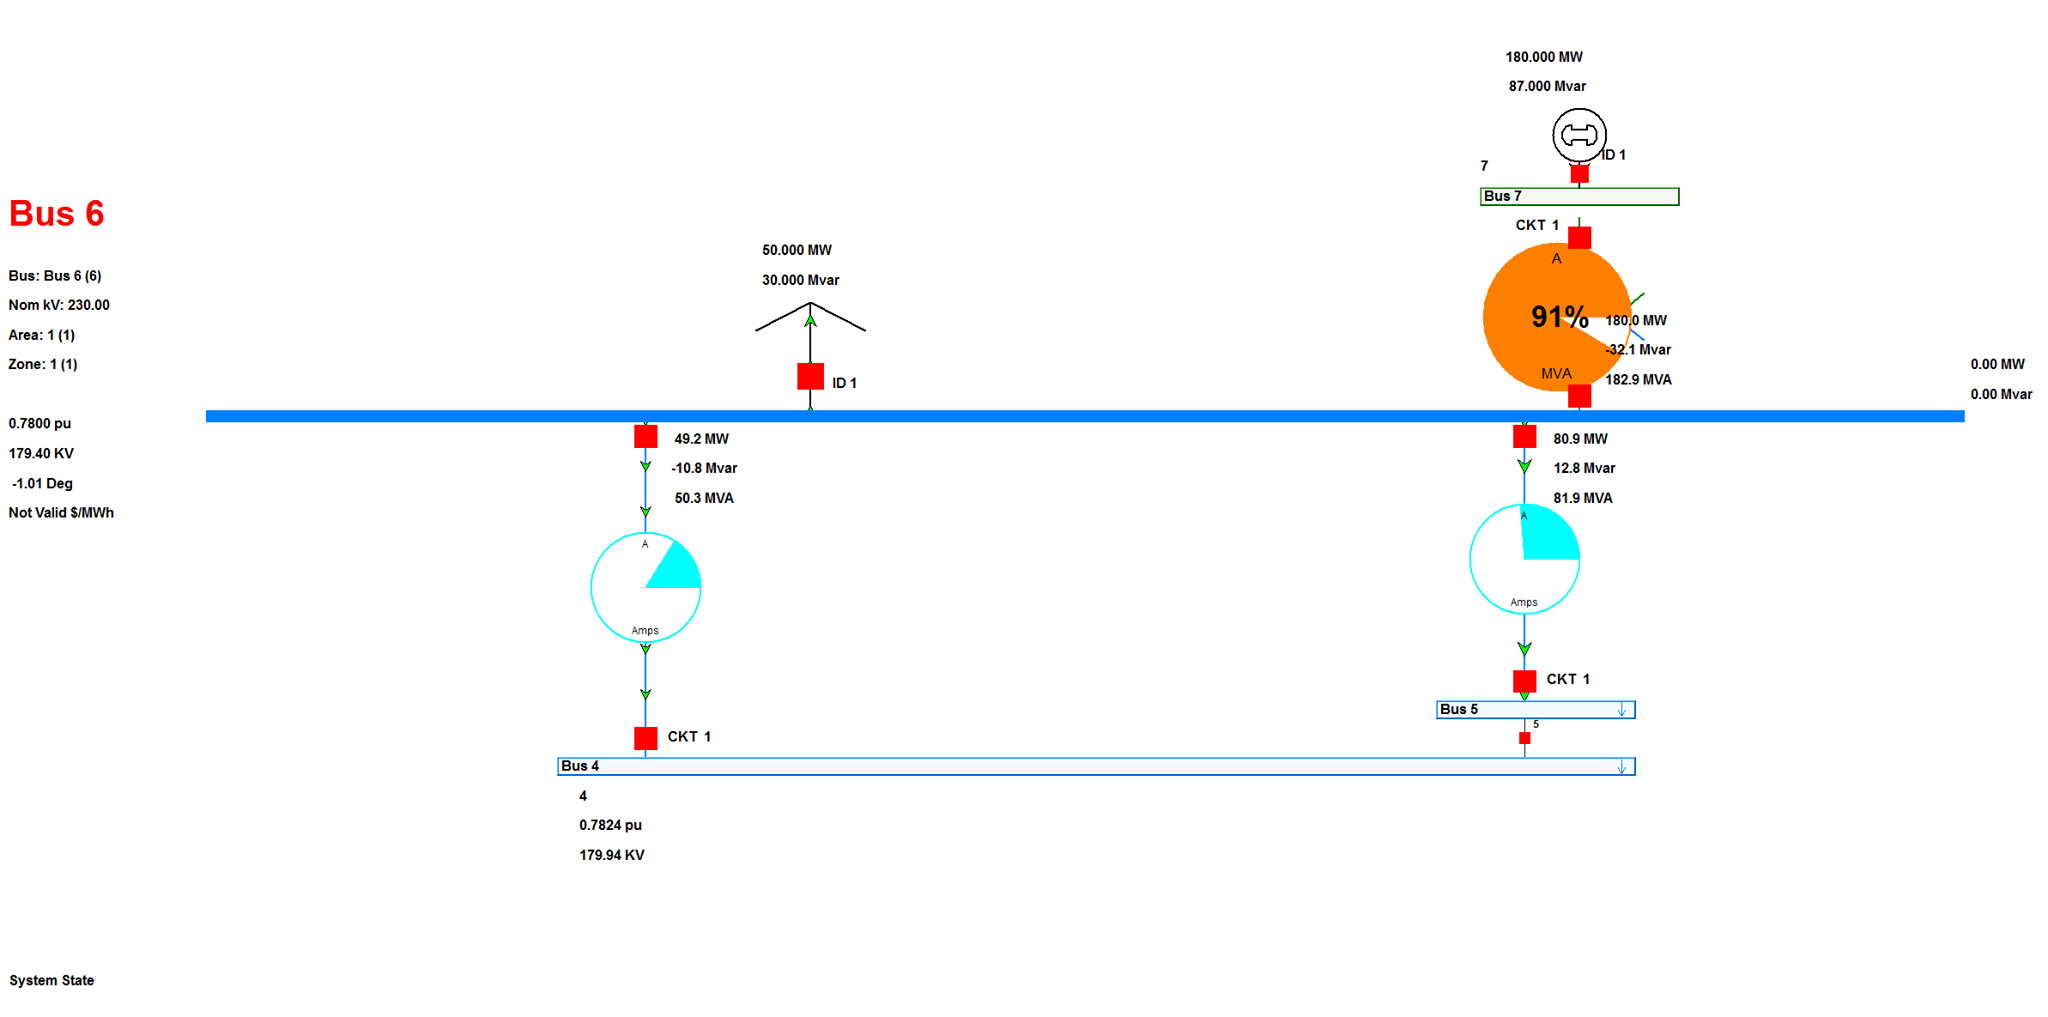
\includegraphics[scale=0.25]{images/PowerWorldBus6}}
            \caption{PowerWorld Diagram - Bus 6 after Newton-Raphson}
        \end{figure}

        \begin{figure}[H]
            \centerline{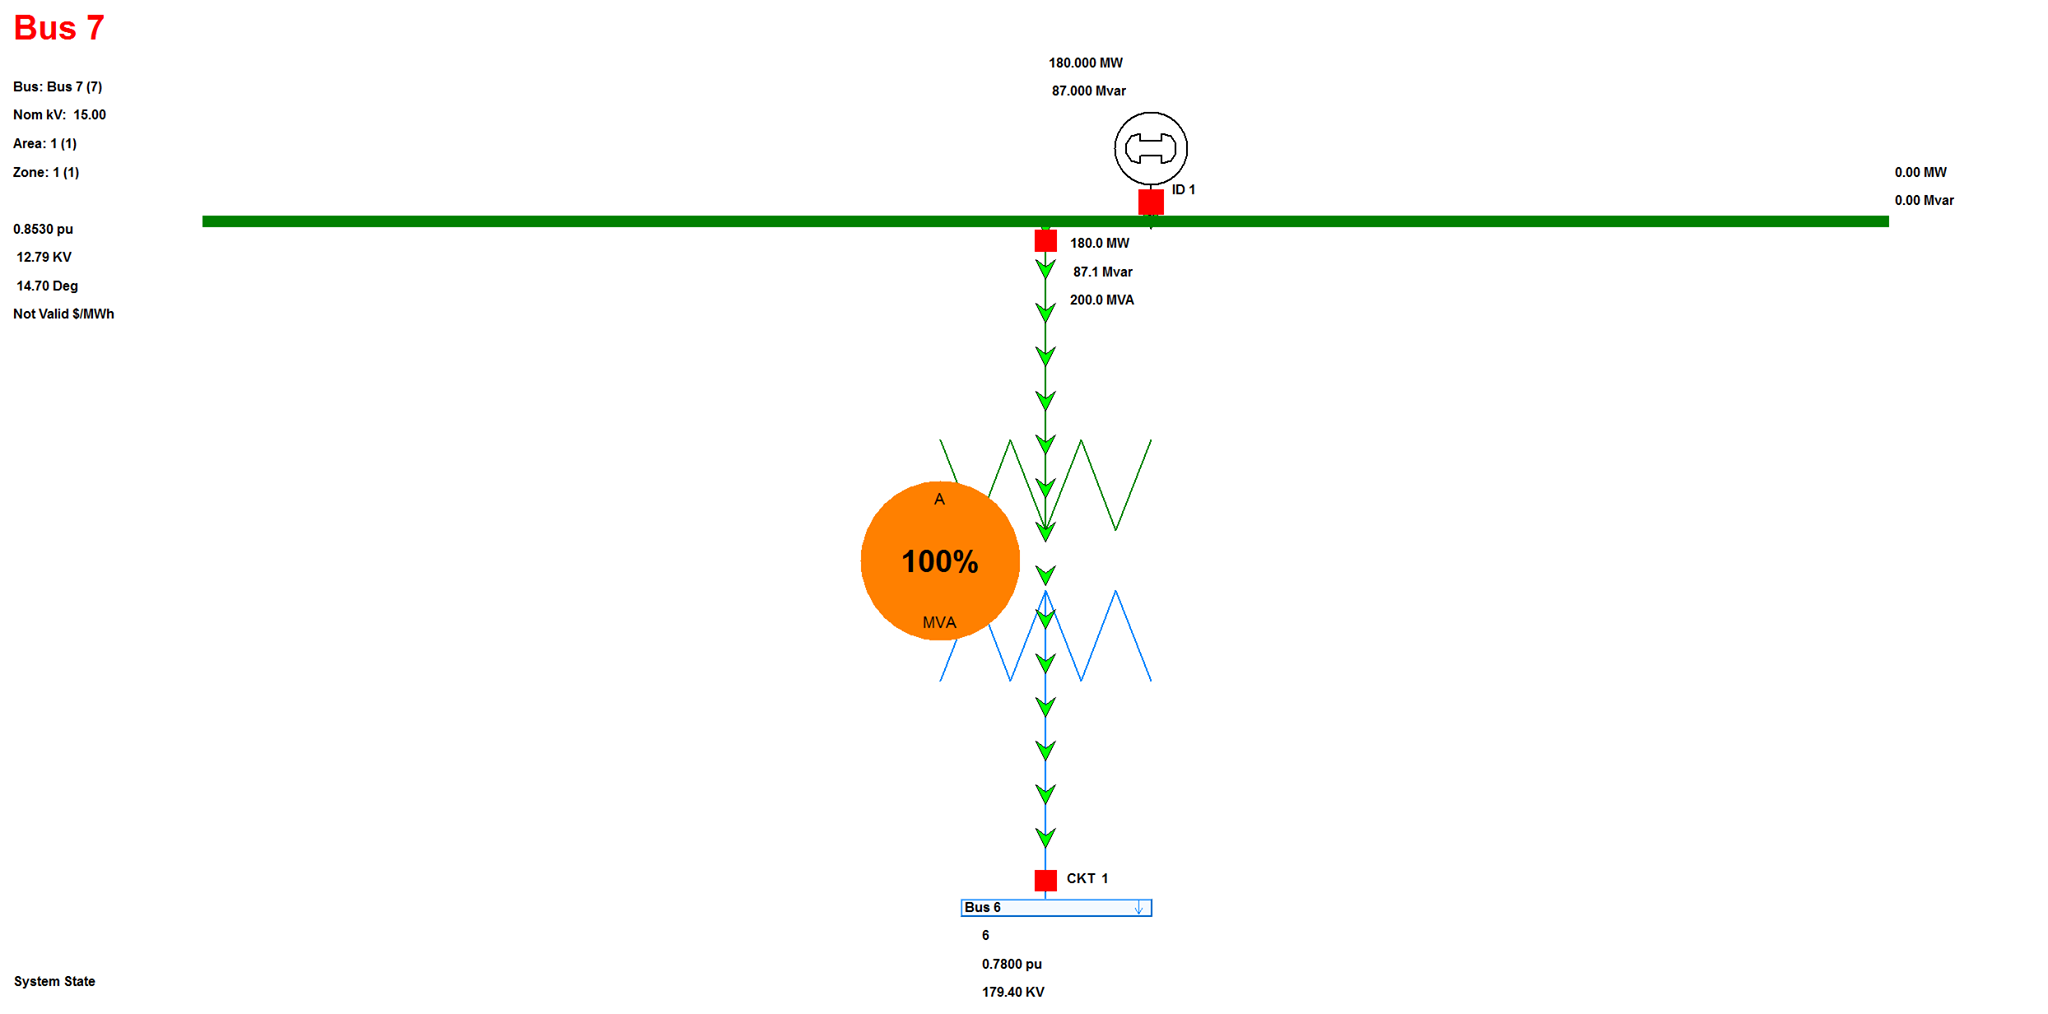
\includegraphics[scale=0.25]{images/PowerWorldBus7}}
            \caption{PowerWorld Diagram - Bus 7 after Newton-Raphson}
        \end{figure}

        \begin{figure}[H]
            \centerline{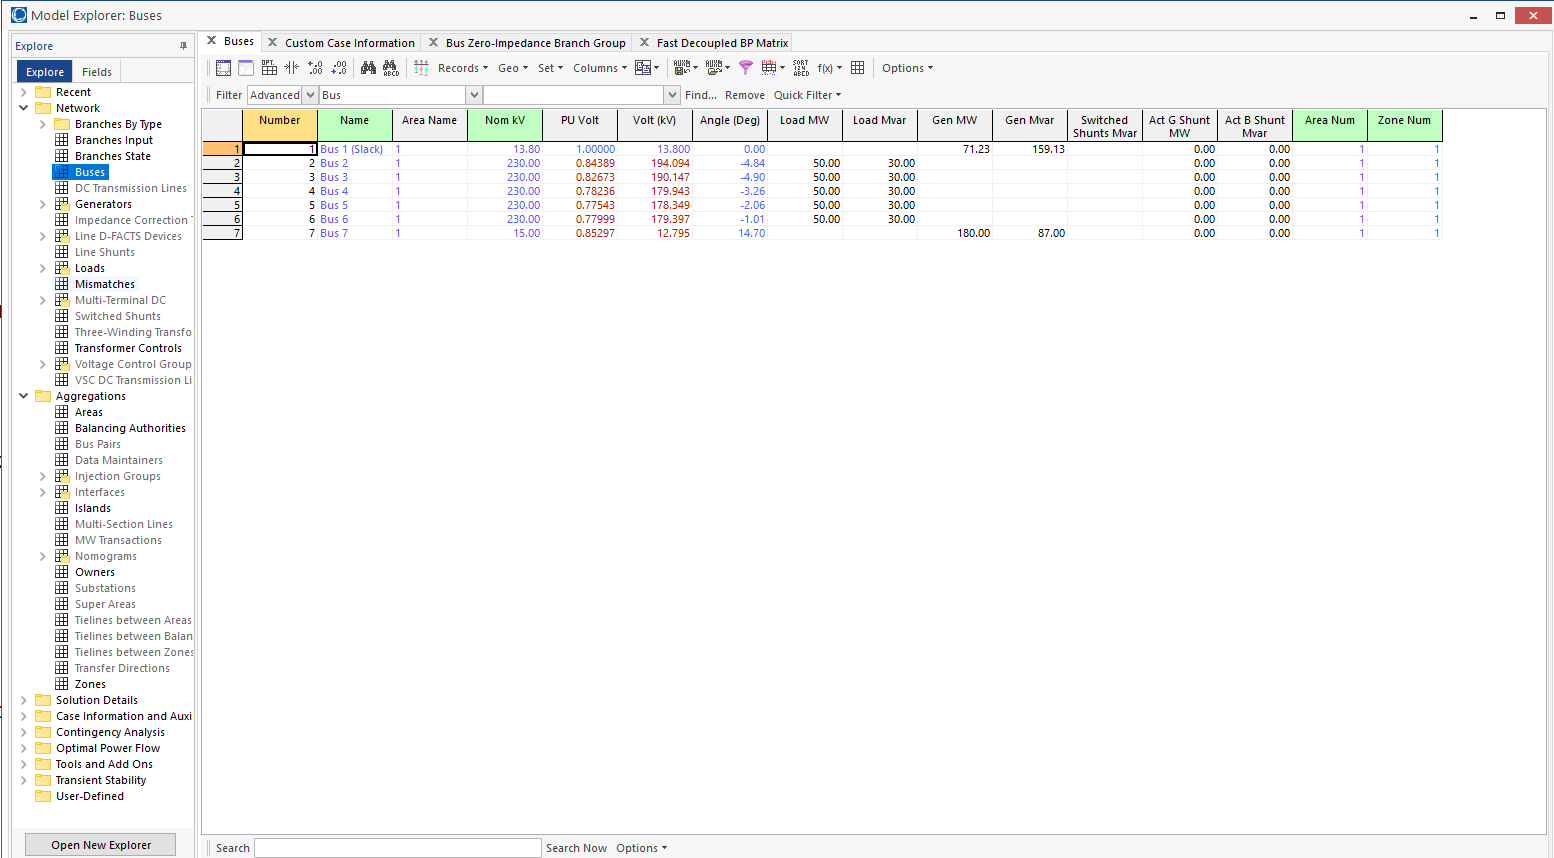
\includegraphics[scale=0.3]{images/PowerWorldTable1}}
            \caption{PowerWorld Diagram - Buses}
        \end{figure}
        \begin{figure}[H]
            \centerline{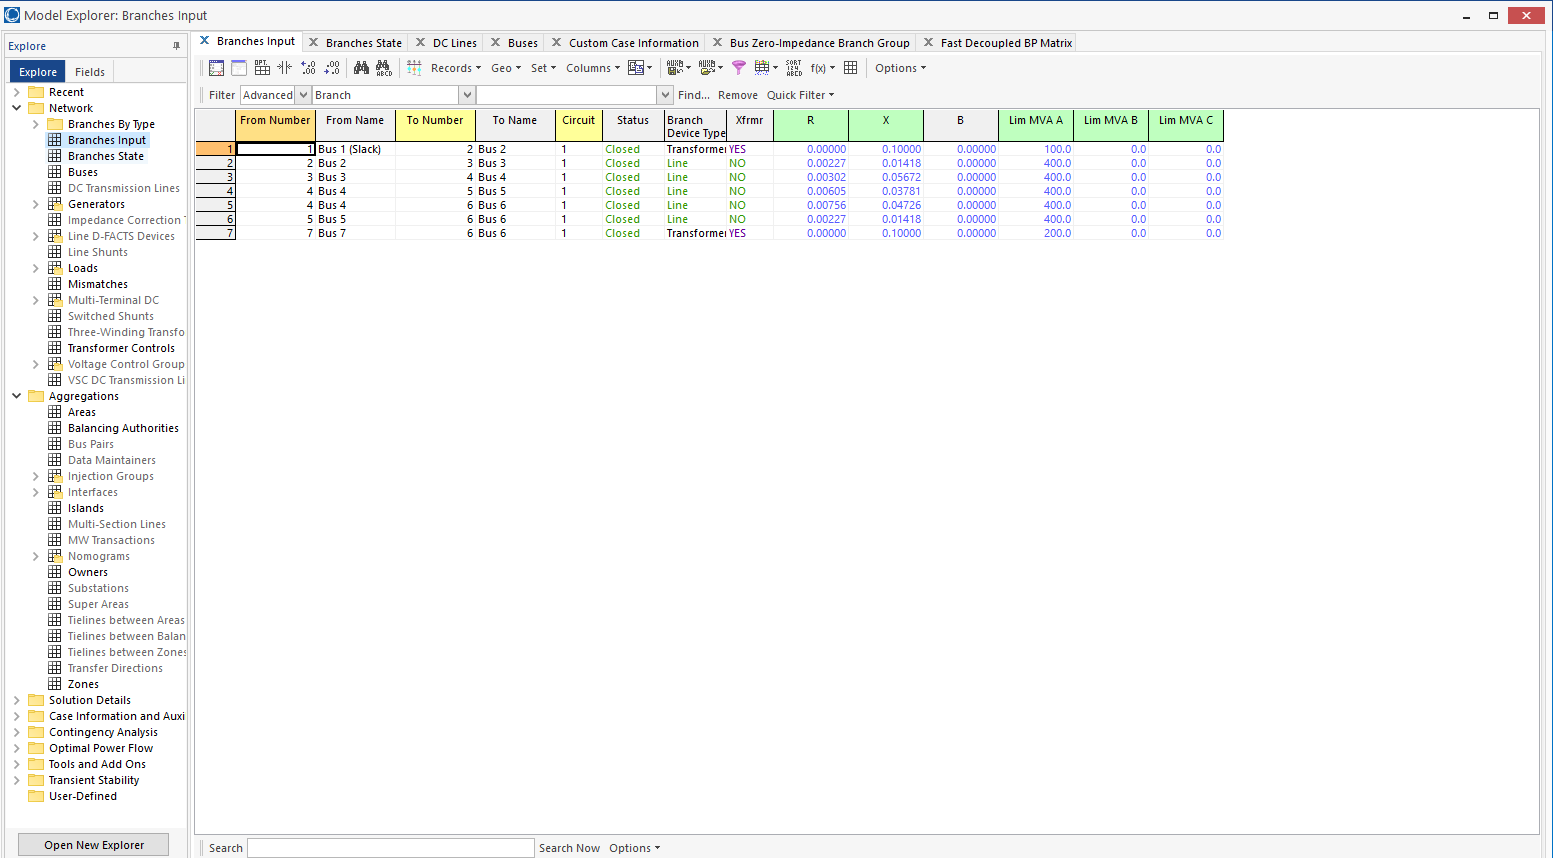
\includegraphics[scale=0.3]{images/PowerWorldTable2}}
            \caption{PowerWorld Diagram - Branch Inputs}
        \end{figure}
        \begin{figure}[H]
            \centerline{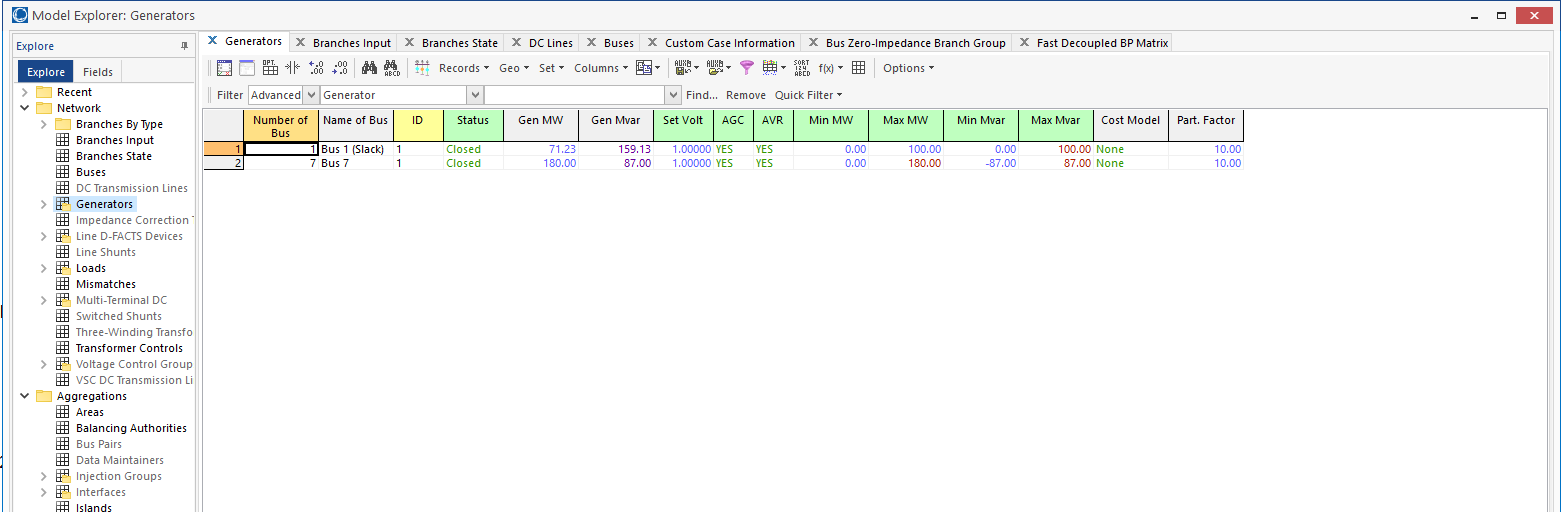
\includegraphics[scale=0.3]{images/PowerWorldTable3}}
            \caption{PowerWorld Diagram - Generators}
        \end{figure}
        \begin{figure}[H]
            \centerline{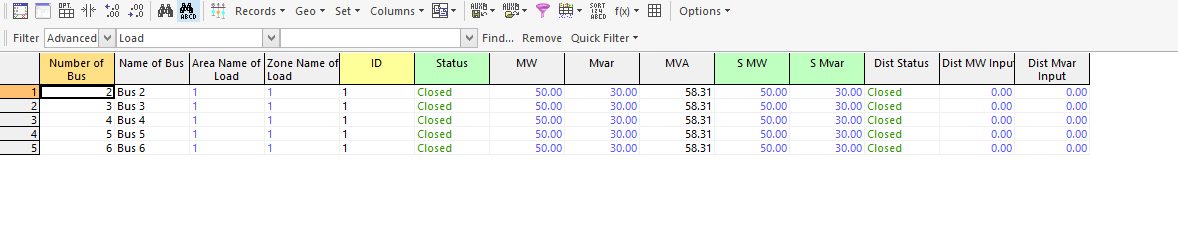
\includegraphics[scale=0.3]{images/PowerWorldTable4}}
            \caption{PowerWorld Diagram}
        \end{figure}
        \begin{figure}[H]
            \centerline{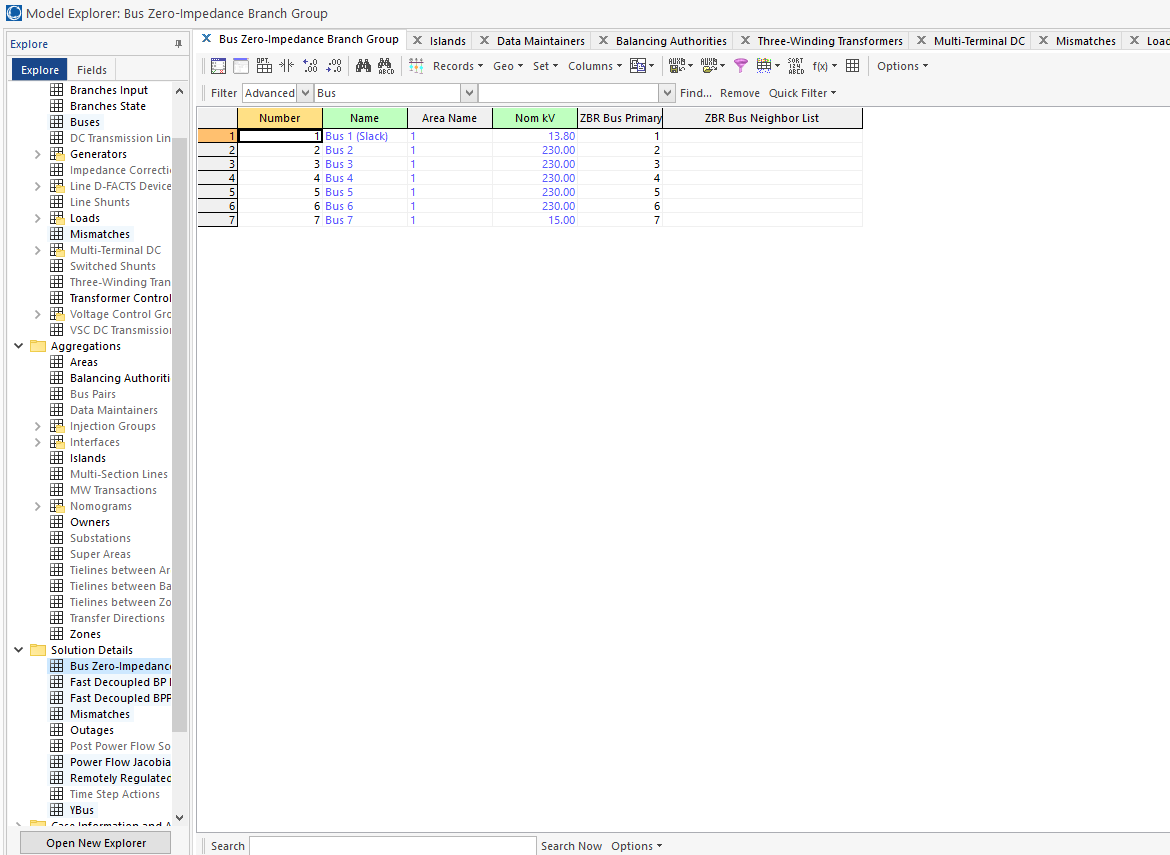
\includegraphics[scale=0.3]{images/PowerWorldTable5}}
            \caption{PowerWorld Diagram - Bus Zero Impedance Branch Groups}
        \end{figure}
        \begin{figure}[H]
            \centerline{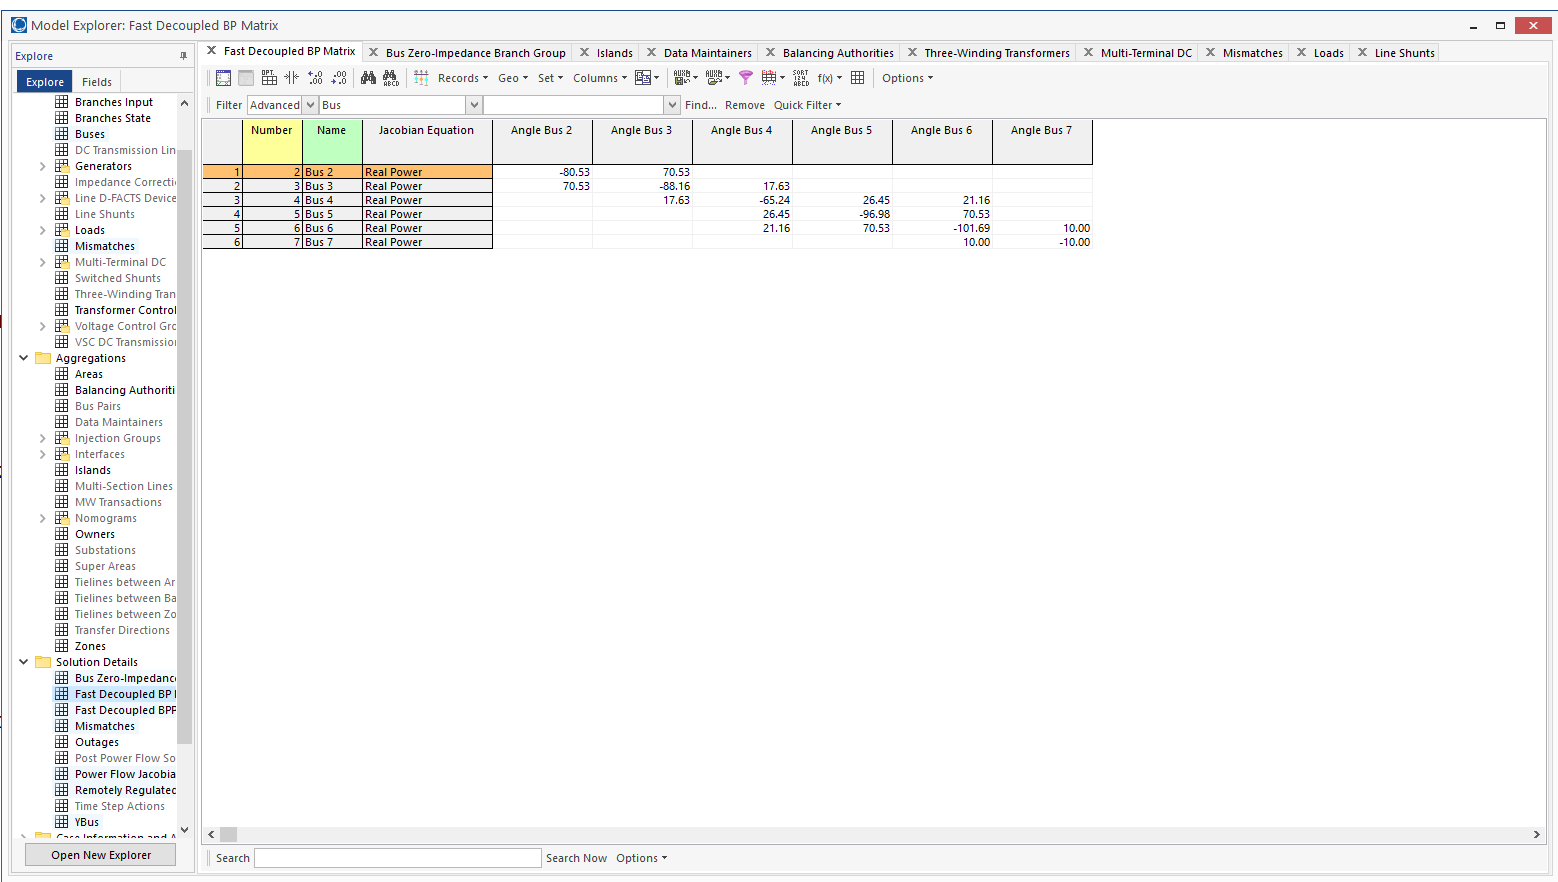
\includegraphics[scale=0.3]{images/PowerWorldTable6}}
            \caption{PowerWorld Diagram - Fast Decoupled BP Matrix}
        \end{figure}
        \begin{figure}[H]
            \centerline{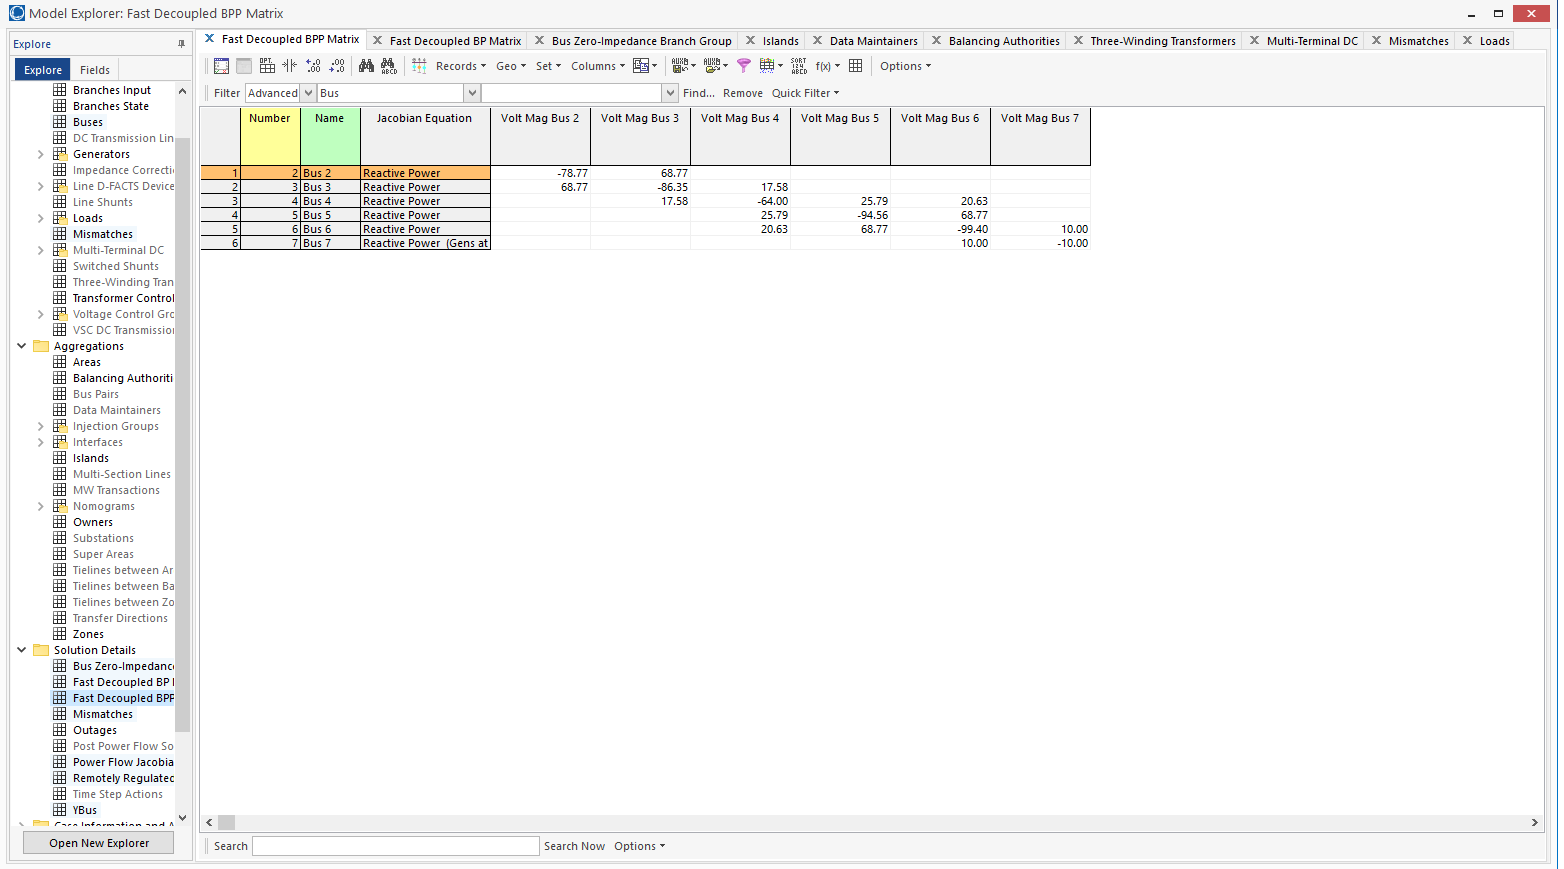
\includegraphics[scale=0.3]{images/PowerWorldTable7}}
            \caption{PowerWorld Diagram - Fast Decoupled BPP Matrix}
        \end{figure}
        \begin{figure}[H]
            \centerline{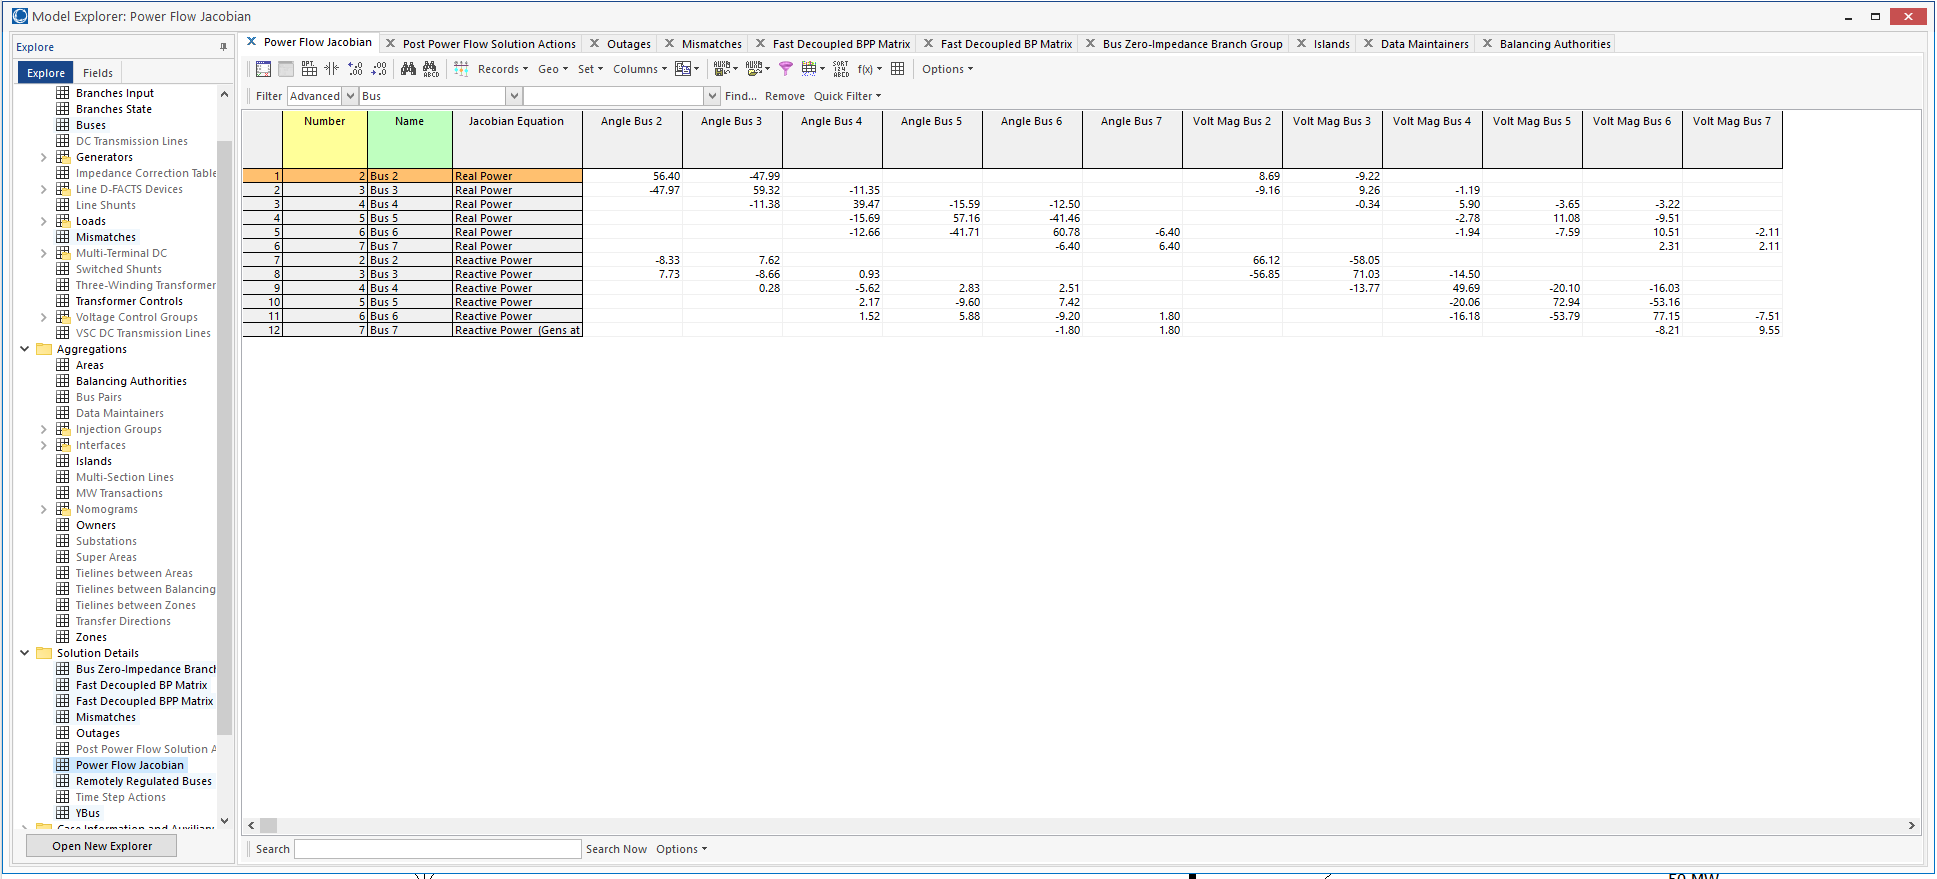
\includegraphics[scale=0.3]{images/PowerWorldTable8}}
            \caption{PowerWorld Diagram - Powerflow Jacobian Matrix}
        \end{figure}
        \begin{figure}[H]
            \centerline{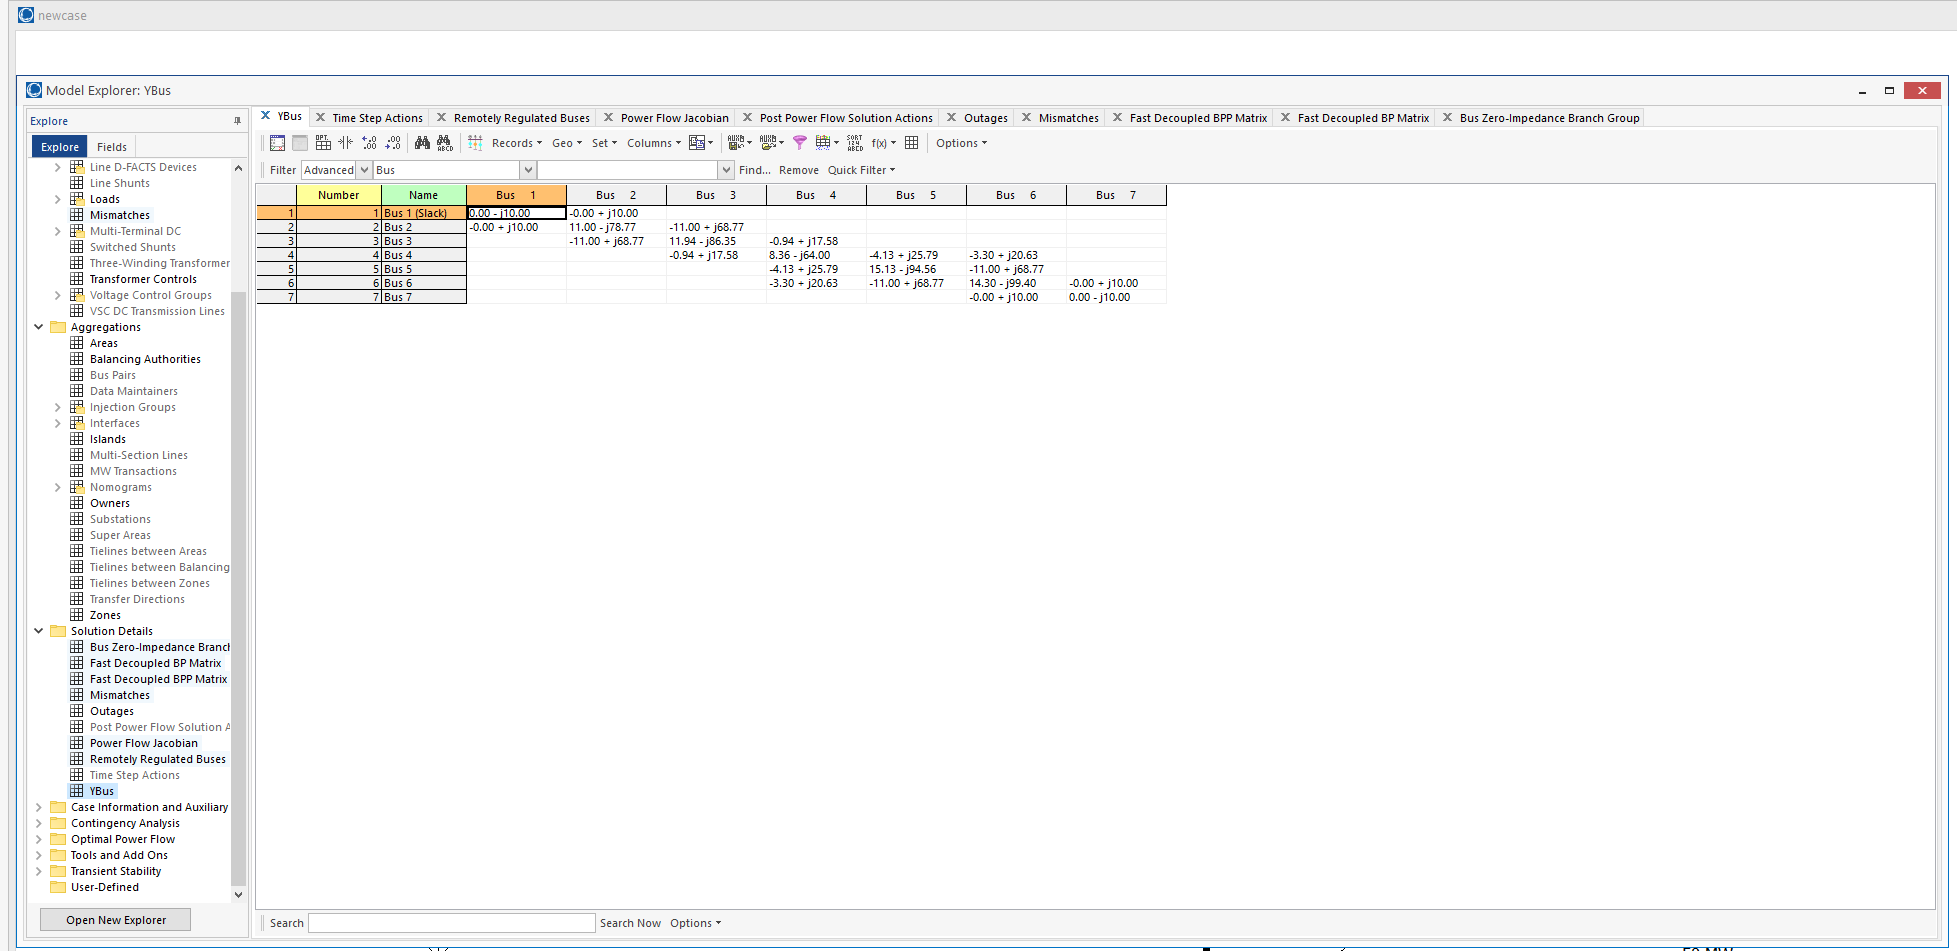
\includegraphics[scale=0.3]{images/PowerWorldTable9}}
            \caption{PowerWorld Diagram - Ybus values}
        \end{figure}

    
        % \subsection{Compute All Power Values}

        \subsection{Compute All Power Values}
         Line losses added in
        % \subsubsection{Compute Power Flow on Each Line (In/Out)}

        \subsubsection{Compute Line Losses}
        $$P_{loss}=\frac{P^2R}{V^2}$$

        @L1
        $$Z=1.2+j7.5\Omega$$
        $$P_{loss}=\frac{100^2\cdot (1.2+j7.5)}{13.8^2}=\frac{12000+j75000}{190.44}=63.01+j393.82$$

        @L2
        $$Z=1.6+j10\Omega$$
        $$P_{loss}=\frac{100^2\cdot (1.6+j10)}{13.8^2}=\frac{16000+j100000}{190.44}=84.02+j525.1$$

        @L3
        $$3.2+j20\Omega$$
        $$P_{loss}=\frac{100^2\cdot (3.2+j20)}{13.8^2}=\frac{32000+j200000}{190.44}=168.03+j1050.2$$

        @L4
        $$1.2+j7.5\Omega$$
        $$P_{loss}=\frac{100^2\cdot (1.2+j7.5)}{13.8^2}=\frac{12000+j75000}{190.44}=63.01+j393.82$$
        
        @L5
        $$4+j25\Omega$$
        $$P_{loss}=\frac{100^2\cdot (4+j25)}{13.8^2}=\frac{40000+j250000}{190.44}=210.04+j1312.75$$
        
        % \subsubsection{Compute Generated Power}
        
        \newpage

        \section{Conclusions}
		\indent\par{What we learned from the PowerWorld simulation is that power flow is slower as we reach the center of the power grid. From the amp meters on the transmission lines we can see that less than 25\% of the maximum handled Amps are being transferred through the line. This is unlike at the generators, where the two transformers T1 and T2 are extremely overpowered. We can also see the per unit voltage present at each bus in the following graph:}
		
		\begin{figure}[H]
			\centerline{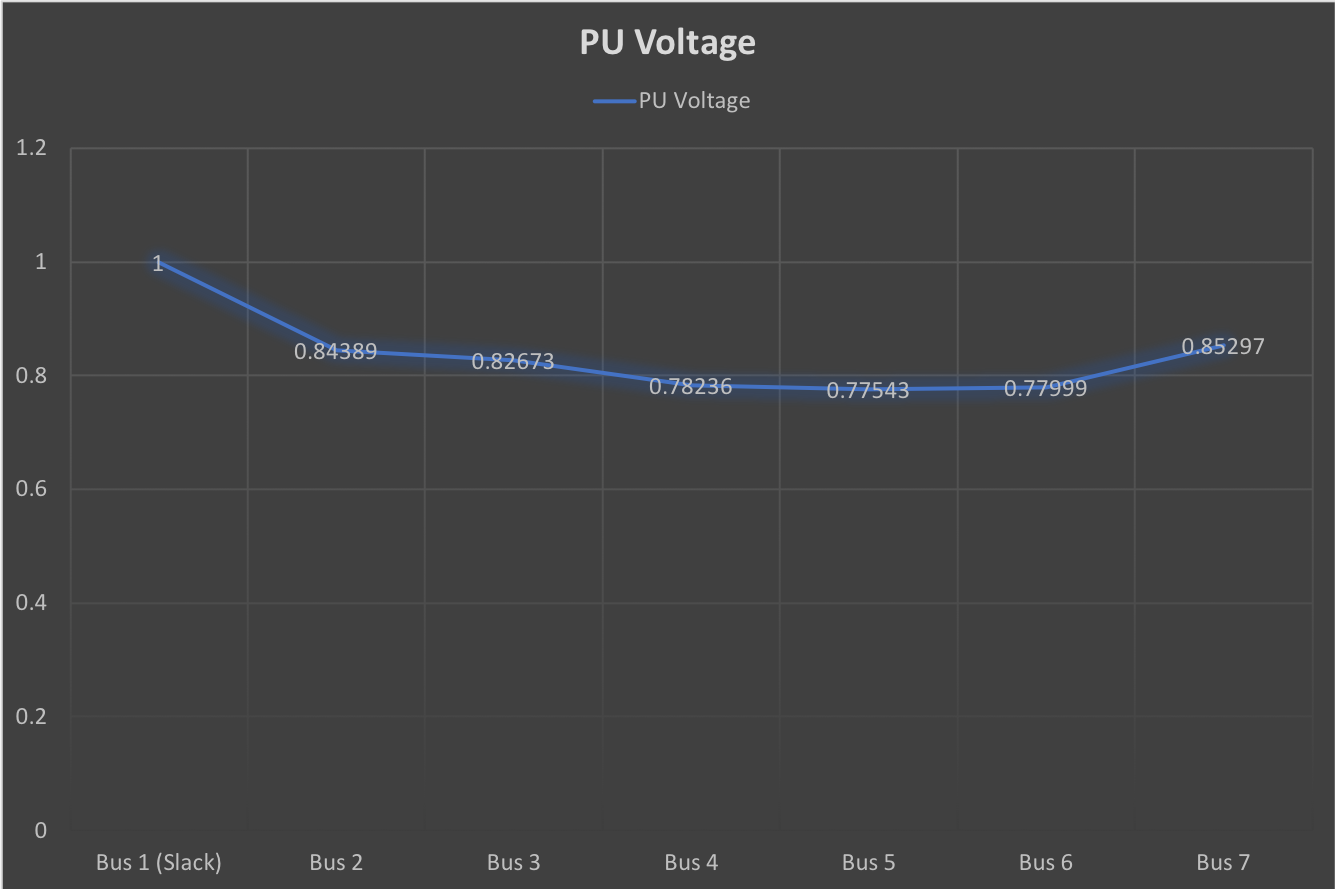
\includegraphics[scale=0.6]{images/perunit}}
			\caption{Per Unit Voltages on buses.}
		\end{figure}
	
	\indent\par{We can also see from the nominal voltage expected to what voltage was simulated at the bus points in the following:}
	\begin{figure}[H]
		\centerline{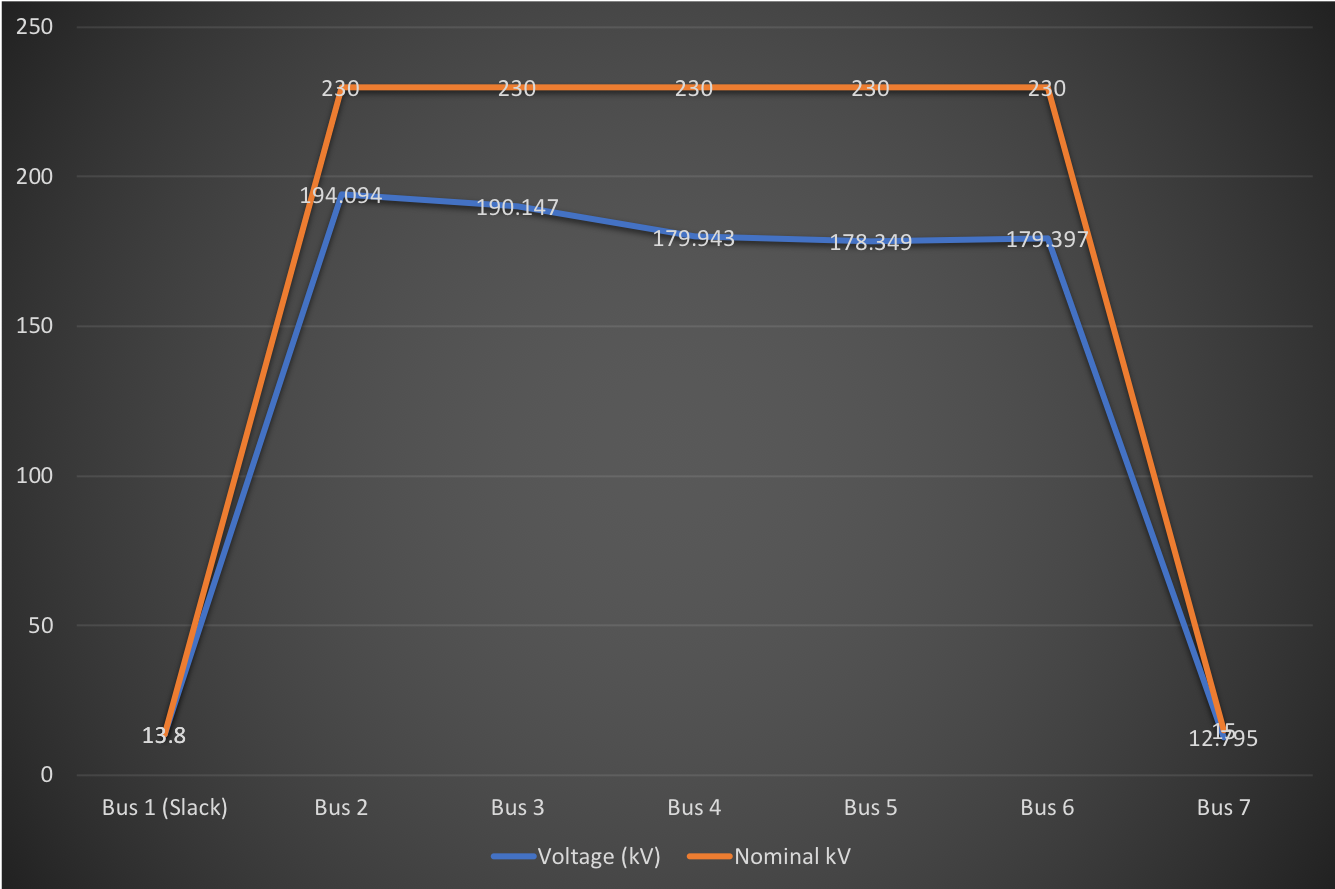
\includegraphics[scale=0.6]{images/nomvsact}}
		\caption{Nominal Voltage vs Actual Voltage of Buses.}
	\end{figure}
		
        % %%%%%%%%%%%%%%%%%%%%%%%%%%%%
        % %%% INCLUDE BIBLIOGRAPHY %%%
        % %%%%%%%%%%%%%%%%%%%%%%%%%%%%
        % \bibliography{Report.bib}
        % \bibliographystyle{ieeetr}
        % \newpage

        % \begin{appendices}
        %     \section{Code}
        % \end{appendices}
    \end{document}   